
\documentclass[a4paper, 12pt, openany]{book} %chose the paper size and font size. Openany ensures that all all chapters and similar may begin at any page, not only odd pages. For the introductory pages and appendices we want openany, but for chapter pages in the main content we want chapters to begin only on odd pages (right hand side). The book class ensures that the margins are automatically adjusted such that left hand pages are slightly moved to the left and vice versa at the right, which makes the thesis very readable and good looking when printed in bound book format.
\usepackage[utf8]{inputenc} %to manage special characters
\usepackage[T1]{fontenc} %to manage special characters
\usepackage[Bjarne]{fncychap} %fancy chapter style (many more available, like Sonny or Lenny etc.)
\usepackage{fancyhdr} %to customize the headers
\usepackage[lmargin=1.5in, rmargin=1in, tmargin=1in, bmargin=1in]{geometry} %sets the margins for the pages
\setcounter{tocdepth}{2} %table of contents number depth for subsections (2 = x.x.x)
\setcounter{secnumdepth}{4} %numbering depth for headers for subsections in the text(4 = x.x.x.x)
\usepackage{url} %to include urls
\usepackage{listings} %include this if you want to include code in the thesis
\usepackage{amsmath,amssymb} %mathematical package
\usepackage{siunitx} %includes SI-units
\usepackage[bf]{caption} %makes float captions bold
\usepackage{array, booktabs} %to make better tables
\usepackage{graphicx} %to include graphics
\usepackage{float} %to include floats
\usepackage[export]{adjustbox} %to adjust floats
\usepackage{subfig} %to include subfigures
\usepackage{chngcntr} %will make it possible to change the counter for tables, figures etc. such as below
\usepackage{color, xcolor} %edit e.g. text colors

\usepackage[backend = biber,
            style = numeric,
            date = long,     % Long: 24th Mar. 1997 | Short: 24/03/1997
            sorting = none,
            maxcitenames = 3,   % max names to include before et. al.
            ]{biblatex} %customize the look of your citations and bibliography
\addbibresource{mybibliography.bib} %declare the bibliography resource
\usepackage{comment} %to be able to comment out sections in the .tex files
\usepackage{afterpage} %to customize page commands such as below
\newcommand\myemptypage{
    \null
    \thispagestyle{empty}
    \addtocounter{page}{-1}
    \newpage
    } %sets new page command to insert an empty page without adding to the page counter or having a page number
\usepackage{setspace}
\setstretch{1.25}
\usepackage{indentfirst}
\usepackage{tabularx}



\begin{document}
%%%%%%%%%%%%%%%%%%%%%%%%%%%%%%%%%%%%%%%%%%%%%%%%%%%%%%%%
%\begin{comment}
% The title page:
% For NTNU students this page will be generated automatically when submitting your paper, and should not be included in the final file from Latex. Delete or comment out the title page setup. The final report should then start with the first page being the abstract. I have included a title page here so it is possible to see how it may look like, and for those who does not get an automatically generated title page. Of course you will need to change the names and titles etc. to your case.

%the title page should be an odd page (right hand side)

\begin{titlepage}
\newgeometry{left=1.6in, right=2in}
\vspace*{1.5cm}

\noindent  \textcolor{gray}{\large Ola Runeson Rasmussen} \\
\vspace{1cm}

\noindent \textbf{\Large Analyzing the Impact of COVID-19 on the Total Points Scored in NBA \newline Basketball Matches:} \\
\vspace{0.5cm}

\noindent {\large A Comparative Study of Pre and Post-Pandemic Seasons} \\



\vspace{5cm}
\noindent Bachelor's thesis in Mathematical Sciences \\
Supervisor: Jarle Tufto \\
June 2023 \\

\vspace{0.1cm}
\noindent Norwegian University of Science and Technology \\
Faculty of Information Technology and Electrical Engineering \\
Department of Mathematical Sciences \\

\begin{figure}[h]
    
\includegraphics[width=0.28\textwidth]{Figures/ntnu_basic.png}
\end{figure}
\end{titlepage}
\restoregeometry
\myemptypage %empty page such that the abstract starts at the first right hand side after the title page
%\end{comment}
%%%%%%%%%%%%%%%%%%%%%%%%%%%%%%%%%%%%%%%%%%%%%%%%%%%%%%%%

% The pre-chapters
\chapter*{Abstract} %pre-chapters should not be numbered, hence the "*"
\pagenumbering{roman} %introductory pages should be roman
\setcounter{page}{1}
\addcontentsline{toc}{chapter}{\protect\numberline{}Abstract} %add the chapter to the table of contents, this is not automatically added when creating unnumbered chapters (*). Add it in a chapter style, and keep all chapters on the same numberline indent regardless of number or not on the chapter

In this thesis I will analyze the impact that the Covid-19 pandemic had on the number of points scored in a NBA basketball match. I will find the model that best fits the data, and analyze the home court advantage and find out if the home court advantage changed during the Covid-19-season. I will also analyze the impact the number of fans present at a match had on the total amount of points obtained by both the home team and opposing team. As a bonus, I will find the strengths of each team throughout the years. \\

I denne oppgaven skal jeg analysere hvilken innvirkning Covid-19-pandemien hadde på antall poeng scoret i en NBA-basketballkamp. Jeg skal finne den modellen som passer best til dataene, og analysere hjemmebanefordelen og finne ut om hjemmebanefordelen endret seg i løpet av Covid-19-sesongen. Jeg vil også analysere hvilken innvirkning antallet tilstedeværende fans på en kamp hadde på det totale antallet poeng oppnådd av både hjemmelaget og motstanderlaget. Som en bonus vil jeg finne styrken til hvert lag gjennom årene.
 %insert the chapter text from the files

\chapter*{Preface}
\addcontentsline{toc}{chapter}{\protect\numberline{}Preface} 

\noindent I would like to thank my supervisor and my family for helping me though this process.


\begin{singlespace}
\tableofcontents
\addcontentsline{toc}{chapter}{\protect\numberline{}Contents}
\end{singlespace}

\newpage
\myemptypage
%add an empty non-counted page by the command below in order to get the first chapter on the left hand side, if needed (check your page number so that the first chapter is on an odd page)


%%%%%%%%%%%%%%%%%%%%%%%%%%%%%%%%%%%%%%%%%%%%%%%%%%%%%%%%
%Customize the layout of the main content of your thesis

\pagestyle{fancy} %set customized page style for header
\fancyhf{} %clear header and footer fields
\renewcommand{\headrulewidth}{0pt} %set to no rule
\fancyhead[LE, RO]{\thepage} %set the page number at left for even, right for odd pages
\fancyhead[RE, LO]{\leftmark} %set the chapter name at right for even, left for odd pages
%is is possible to design the header with the chapter as you wish, e.q. only the chapter or only the name, all lowercase instead etc.
%you could also design the footer if you wish, for example:
%\fancyfoot[LE, RO]{\thepage}
\setlength{\headheight}{14.49998pt} %set the header height


%%%%%%%%%%%%%%%%%%%%%%%%%%%%%%%%%%%%%%%%%%%%%%%%%%%%%%%%
%main content 

\pagenumbering{arabic}
\chapter{Introduction}

\section{Modelling Sports Results}

\noindent Modelling sport results can have many different use cases. It can be used to predict future matches, player performance among other things. Coaches and analysts can use data to analyze strengths and weaknesses of players and opponents, and scouts can use models to find what players could have a potential future in that sport. The main objective of this thesis is to find a model that fit 8 seasons worth of data from the National Basketball Association (NBA), starting with the 2014-2015 season, skipping the 2019-2020 season, and ending with the 2022-2023 season. The reason why the 2019-2020 season is skipped is because this season got cut short because of the covid-19-pandemic. Something similar has been done in \cite{fotballglmm}, were they modelled the scores in football matches to find the attack strength and defence strength of teams, but they also found the home-field advantage that a team has. In this thesis I will also find the home-court advantage but also find the differences between the 2020-2021 season and the other seasons. Due to covid restrictions, this season was played without any fans, so it will be interesting to see if the home-court advantage disappeared or got weaker. Further differences between what they have done and what I have done in this thesis will be looked at in Section \ref{bestmod}. \\

\newpage

\section{NBA}

\noindent The NBA, National Basketball Association, is the biggest basketball league in North-America. A regular season in the NBA, consists of 82 games for each team. There are 30 teams in the NBA, divided into 2 conferences, the eastern- and the western conference. Teams in the same conference plays 4 games against each other and 2 games against teams in the other conference. The 2020 to 2021 season, reffered to as the Covid season, only consisted of 72 games for each team. Also, under this season there where no fans allowed because of Covid-19 regulations.

There are 3 different scoring methods, or types, in a normal NBA game. You have the one-pointers, scoring method one, which are scored from free throws. Free throws are a form of penalties obtained when the other team commits a foul. Two-pointers, scoring method two, are obtained from getting the basketball into the opponents hoop while inside the three point line, while three-pointers, scoring method three, are obtained from scoring outside the three point line. Also, a team is awarded 2 free throws when fouled while attempting a two pointer, and 3 free throws when fouled while attempting a three pointer. But they are only awarded 1 free throw if they scored while being fouled.

\section{Home Court Advantage}

\noindent In \cite{homecourtadv}, the author analyzed home court advantages for NCAA basketball statistics. NCAA, National Collegiate Athletic Association, is the college equivalent of the NBA. He came to the conclusion that when playing on their home court, a team received a boost in nearly all statistical categories. In this thesis, I will come to the same conclusion that teams scored more points while playing on their home court.

\cleardoublepage
%the cleardoublepage command ensures that the next text page is on the right-hand side (odd page) and produces a blank page if necessary to achieve that, as all chapters should begin on the right hand side


\chapter{Theory}

\section{Generalized linear Models}

\noindent All of this theory is collected from \cite{regression} if not stated otherwise. In a Generalized linear Model (GLM), where we have $i = 1, 2, \dots, n$ observations, we want to find a linear relationship between the covariate vectors, the $\mathbf{x}_i$'s, and a transformation of the expected value, mean $\mu_i$, of a distribution. That is,

\begin{equation}
g(\mu_i) = \eta_i = \mathbf{x}_i^\top \boldsymbol{\beta}.
\label{eqn:Link}
\end{equation}

\noindent where $g(\mu_i)$, the link function, is the function that transforms this into a linear relationship, and $\eta_i = \mathbf{x}_i^\top \boldsymbol{\beta}$ is called the linear predictor. There are many different link functions for different distributions. One thing these distributions have in common is that they are a part of the Exponential Family of distributions. The probability mass function of a multivariate exponential family for the response variable $y_i$ is defined by,

\begin{equation}
f(y_i|\theta_i) = exp\Biggl\{ \frac{y_i\theta_i - b(\theta_i)}{\phi} w_i + c(y_i,\phi,w_i) \Biggr\},
\label{eqn:ExpFam}
\end{equation}

\noindent where the parameter $\theta_i$ is called the natural or canonical parameter, the parameter $\phi$ is the dispersion parameter, and $w_i$, usually a weight, is a known value. For the function $b(\theta_i)$, it is required that $f(y_i|\theta_i)$ can be normalized and that $b'(\theta_i)$ and $b''(\theta_i)$ exist. The expected value and variance of this probability mass function is then defined by,

\begin{equation*}
E[y_i] = \mu_i = b'(\theta_i), \ \ Var[y_i] = \sigma_i^2 = \phi \frac{b''(\theta_i)}{w_i}.
\label{eqn:EV}
\end{equation*}

\section{Generalized linear Mixed models }

\noindent Generalized linear Mixed models (GLMMs) are defined by adding a random effect $\boldsymbol{\gamma}_i$ to the linear predictor $\eta_i = \mathbf{x}_i^\top \boldsymbol{\beta}$. The responses $y_{ij}$, where $i = 1,\dots,m$, $j = 1, \dots, n_i$, with $n_i$ being the measurements per individual or cluster. When adding a cluster specific random effect $\boldsymbol{\gamma}_i$ to the responses $y_{ij}$, the conditional mean $\mu_{ij} = E[y_{ij}|\gamma_i]$ is linked to the linear predictor,

\begin{equation}
\eta_{ij} = \mathbf{x}_{ij}^\top \boldsymbol{\beta} + \mathbf{u}_{ij}^\top \boldsymbol{\gamma}_i, \ \ \ \ i = 1,\dots,m, \ \ \ \ j = 1, \dots, n_i,
\label{eqn:LinPredGLMM}
\end{equation}

\noindent through the link function $g(\mu_{ij}) = \eta_{ij}$. Here the random effects $\gamma_i$ are independent and identically distributed $N(0,Q)$ where $Q$ is the covariance matrix for the random effects \cite{regression} p. 391. To estimate these fixed and random effects, I will use the "glmmTMB" package in R. Simply said, this package will numerically approximate the estimated values.

\section{Poisson process}

\noindent One distribution that is a part of the exponential family of distributions, is the Poisson distribution. It is defined by the density,

\begin{equation}
f(y_i|\lambda_i) = \frac{\lambda_i^{y_i} e^{-\lambda_i}}{y_i!}, \ \ y_i = 0,1,\dots,
\label{eqn:expPDF}
\end{equation}

\noindent where $y_i$ is the total amount of times an event occurs in an interval, and $\lambda_i > 0$ is the rate at which the occurrences happen. In this thesis I will model the scores in a basketball match via a Poisson process. The mean and variance of the Poisson distribution is the same. That is,

\begin{equation*}
E[y_i] = \mu_i = \lambda_i, \ \ Var[y_i] = \lambda_i.
\label{eqn:expEV}
\end{equation*}

\noindent The natural link function to use for the Poisson distribution is the log-link function, which is given by,

\begin{equation}
g(\lambda_i) = \log(\lambda_i) = \eta_i = \mathbf{x}_i^\top \boldsymbol{\beta}.
\label{eqn:explink}
\end{equation}

\noindent This assures us that the rate $\lambda_i > 0$ for all $\beta \in \Re^p$. The Mixed Poisson model with the log-link function is called the mixed log-linear Poisson model. It is defined as seen below where $y_{ij}|\boldsymbol{\gamma}_i \sim \text{Poisson}(\lambda_{ij})$, where

\begin{equation}
\log(\lambda_{ij}) = \mathbf{x}_{ij}^\top \boldsymbol{\beta} + \mathbf{u}_{ij}^\top \boldsymbol{\gamma}_i.
\label{eqn:logLinkGLMM}
\end{equation}

\noindent In this thesis, the random effects I will use is attack strength $\gamma_{A,i,k}$ and defence strength $\gamma_{D,i,k}$. The notation,

\begin{equation}
\log(\lambda_{ijk}) = "\text{fixed effects}"_k + \gamma_{A,i,k} + \gamma_{D,j,k},
\label{eqn:logLinkGLMMbasket}
\end{equation}

\noindent will be used where $i$ is the attacking team, $j$ is the defending team, and $k$ is the scoring type.

A Poisson process is a continous time process, where events happen independently of one another with a certain rate (intensity) $\lambda$. The probability of $n$ scores in a match is then, 

\begin{equation}
P\big((\text{\# scores of type } k) = n\big) = \frac{\lambda^n}{n!} e^{-\lambda}.
\label{eqn:poipro}
\end{equation}

\noindent In \cite{poissonNBA}, the authors comes to the conclusion that the scores in a basketball match can mostly be seen as a Poisson process, but in close games, the Poisson process assumption breaks. This will be discussed further in Section \ref{future}. In this thesis, I will assume that the scores follow a Poisson process. 

\section{AIC}

\noindent Akaike Information Criterion (AIC) is an estimator for the quality of our model given our data. It penalizes complex models by taking the amount of estimated parameters into account. The formula for AIC is,

\begin{equation}
\text{AIC} = 2k - 2 ln(\hat{L}),
\label{eqn:AIC}
\end{equation}

\noindent where $k$ is the number of estimated parameters and $\hat{L}$ is the maximized value of the likelihood function of our model. The AIC is an estimator for the Kullback Leibler distance between the actual and "true" model. The data will generate an unknown distribution, so the difference between the poisson distribution used and this unknown distribution is then the Kullback Leiber distance, showing how different these two distributions are \cite{kullback}. I will use this criteria to find the best model for the Covid season and the other seasons.

\newpage

\section{Likelihood Ratio Test (LRT)}

\noindent Together with the AIC of a model, the likelihood ratio Test is also used to find significant variables in a model. When testing the hypothesis $H_0: \ \beta = 0$ vs. $H_1: \ \beta \neq 0$, we can use the (log-)likelihood ratio statistic,

\begin{equation}
\text{lr} = 2\big\{ l(\hat\beta) - l(\tilde\beta) \big\} = -2\big\{ l(\tilde\beta) - l(\hat\beta) \big\},
\label{eqn:lrs}
\end{equation}

\noindent where $l(\tilde\beta)$ is the log-likelihood for the restricted model under $H_0$ and  $l(\hat\beta)$ is the log-likelihood of the full model \cite{regression} p. 662-663\\

\section{AR(1)-process}

\noindent An AR(1), auto-regressive, process is a stochastic random process. The AR(1) process $\{X_t\}_{t \in Z}$ is defined as a causal stationary series satisfying the equation,

\begin{equation}
X_t = \varphi X_{t-1} + \epsilon_t, \ \ t = 1,2,\dots,
\label{eqn:ar1}
\end{equation}

\noindent where $|\varphi| < 1$ and $\epsilon_t$ is the white noise with zero mean and variance $\sigma^2_\epsilon$. They are identically and independently distributed \cite{timeseries} p. 15.

\section{OU-process}

\noindent A stationary Gaussian Ornstein-Uhlenbeck process, Gaussian continuous-time AR(1) process, is considered as the continuous-time analogue of the discrete-time AR(1) process, \cite{timeseries} p.343. It can have irregular timepoints instead of the constant even time differences in the AR(1) process. The OU-process $\{U_t\}_{t \in R}$ is defined by the stochastic differential equation,

\begin{equation}
dU_t = -\theta U_t dt + \sigma dW_t,
\label{eqn:ou}
\end{equation}

\noindent where $\theta > 0$, $\sigma > 0$ are parameters and $U_t \sim N\big(u_o e^{-\theta t}, \frac{\sigma^2}{2\theta}\big\{1 - e^{-2\theta t}\big\}\big)$ \cite{IBE2013263}. ${W_t}$ is the Wiener process, which is a two-sided Brownian motion \cite{voutilainen_viitasaari_ilmonen_2019}. An important property of \ref{eqn:ou} is that the autocovariancefunction decreases exponentially.

\cleardoublepage


\chapter{Method}

\section{Collecting Data}

\noindent All of the data used in this thesis is collected from the official NBA website and Basketball Reference seen below:

\begin{itemize}
  \item \url{https://www.nba.com/stats/teams/boxscores-traditional}
  \item \url{https://www.basketball-reference.com/}.
\end{itemize}

\section{Data management}

\noindent All the data was changed into the format seen in Table \ref{table:dataSaved}. Attacking team $i$ is the team attacking defending team $j$, $y$ is the number of scores obtained, type is the scoring type, i.e. when type 3 means three pointer and so on. Home court is "yes" if attacking team $i$ is playing on their home court. Date shows the number of days after the first game saved in the data. Win shows what team won the match. Covid indicate whether we are looking at the Covid season or a normal season, and Number of fans says how many fans were present.

\begin{table}[H]
\centering
\begin{tabular}{ |p{1.8cm}|p{1.8cm}|p{.5cm}|p{1cm}|p{1cm}|p{1cm}|p{1cm}|p{1cm}|p{1.5cm}|  }
    \hline
    Attacking Team $i$ & Defending Team $j$ & $y$ & Type & Home Court & Date & Win & Covid & Number of Fans \\
    \hline
    LAL & HOU & $3$ & $3$ & yes & $1$ & no & no & $18997$ \\
    LAL & HOU & $25$ & $2$ & yes & $1$ & no & no & $18997$ \\
    LAL & HOU & $31$ & $1$ & yes & $1$ & no & no & $18997$ \\
    \hline
    HOU & LAL & $12$ & $3$ & no & $1$ & yes & no & $18997$ \\
    HOU & LAL & $19$ & $2$ & no & $1$ & yes & no & $18997$ \\
    HOU & LAL & $34$ & $1$ & no & $1$ & yes & no & $18997$ \\
    \hline
\end{tabular}
\caption{Six rows of the data frame containing data for one match between the Los Angeles Lakers and the Houston Rockets}
\label{table:dataSaved}
\end{table}

\section{Model Selection Method}

\noindent To find the best model, I used the covariates Type, Home, and Covid. Type is the scoring type, Home is the home advantage, and Covid indicate the covid season. I made many different combinations of these covariates with different interactions and compared them using their AIC value. If two models had the same AIC, i used the Likelihood Ratio Test to find significant terms. These models can be seen in Table \ref{table:AICchangeCovid}.

\cleardoublepage


\chapter{Results and Discussion}

\section{Model Selection} \label{modsel}

\begin{table}[H]
\centering
\begin{tabular}{ |p{1.5cm}|p{8cm}|p{3cm}| }
    \hline
    Models: & Change from the best model: & $\Delta AIC$ from the best model \\
    \hline
    Mod1 &$-\beta_\text{HC} \ x_\text{HC,ij\text{k}} + \beta_\text{HC,\text{k}} \ x_\text{HC,ij\text{k}}$ & $0$ \\
    \hline
    Mod2 &$-\beta_\text{HC} \ x_\text{HC,ij\text{k}}$ & $3$ \\
    \hline
    Mod3 &$-\beta_{\text{C},\text{k}} \ x_\text{C,ij\text{k}} + \beta_{\text{C}} \ x_\text{C,ij\text{k}}$ & $958$ \\
    \hline
    Mod4 &$-\beta_{\text{H},\text{k}} \ x_\text{H,ij\text{k}} + \beta_{\text{H}} \ x_\text{H,ij\text{k}}$ & $14$ \\
    \hline
    Mod5 &$-\beta_{\text{C},\text{k}} \ x_\text{C,ij\text{k}} - \beta_\text{HC} \ x_\text{HC,ij\text{k}} + \beta_{\text{C}} \ x_\text{C,ij\text{k}}$ & $961$ \\
    \hline
    Mod6 &$-\beta_{\text{H},\text{k}} \ x_\text{H,ij\text{k}} - \beta_{\text{C},\text{k}} \ x_\text{C,ij\text{k}} + \beta_{\text{H}} \ x_\text{H,ij\text{k}} + \beta_{\text{C}} \ x_\text{C,ij\text{k}}$ & $972$ \\
    \hline
    Mod7 &$-\beta_{\text{H},\text{k}} \ x_\text{H,ij\text{k}} - \beta_\text{HC} \ x_\text{HC,ij\text{k}} + \beta_{\text{H}} \ x_\text{H,ij\text{k}}$ & $16$ \\
    \hline
    Mod8 &$-\beta_{\text{H},\text{k}} \ x_\text{H,ij\text{k}} - \beta_{\text{C},\text{k}} \ x_\text{C,ij\text{k}} - \beta_\text{HC} \ x_\text{HC,ij\text{k}} + \beta_{\text{H}} \ x_\text{H,ij\text{k}} + \beta_{\text{C}} \ x_\text{C,ij\text{k}}$ & $974$ \\
    \hline
\end{tabular}
\caption{Change in AIC from the best model}
\label{table:AICchangeCovid}
\end{table}

\noindent The best model can be seen in Equation \ref{eq:bestmodelcovid}, but below I will show some neighboring models to the best one that I compared it to in Table \ref{table:AICchangeCovid} along with the difference between the AIC for the best model and these neighboring models. In model $1$, the interaction between the home court advantage and covid is replaced with a three way interaction between home court advantage, covid and each scoring type. In model $2$, the interaction between the home court advantage and covid is removed. In model $3$, the interaction between covid and each scoring type is replaced with a single covid term. In model $4$, the interaction between home court advantage and each scoring type is replaced with a single home court term. Model 5 is almost the same as model 3 but the interaction between home court and covid is removed. Model 6 has both the interaction between home court and scoring type and the interaction between covid and scoring type replaced with just one term for home court and one term for covid. Model 7 is similar to model 4, but the interaction between home court and covid is removed. Finally, model 8 is the same as model 6 but the interaction between home court and covid is removed.

\section{Best Model} \label{bestmod}

\noindent After a great deal of testing, I have found that the best model to use for this data is,

\begin{equation}
    \log(\lambda_{i,j,\text{k}}) = \beta_\text{k} + \beta_{\text{H},\text{k}} \ x_\text{H,ij\text{k}} + \beta_{\text{C},\text{k}} \ x_\text{C,ij\text{k}} + \beta_\text{HC} \ x_\text{HC,ij\text{k}} + \gamma_{\text{A},i,\text{k}} + \gamma_{\text{D},j,\text{k}}.
\label{eq:bestmodelcovid}
\end{equation}

\noindent The scoring type is denoted by index $\text{k} = 1,2,3$, the attacking team is denoted by index $i$, and the defending team is denoted by index $j$. $x_\text{H,ij\text{k}}$, $x_\text{C,ij\text{k}}$, and $x_\text{HC,ij\text{k}}$ are dummy, or indicator, variables. They indicate if we have a match where attacking team $i$ has home court advantage, if we have a match played during the Covid-season, or if we have a match with home court advantage during the Covid-season, respectively. Table \ref{table:fixedEffCovid} shows the fixed effects of the model in Equation \ref{eq:bestmodelcovid} together with their standard deviations, and Table \ref{table:fixedEffExpCovid} shows the percent the expected number of scores changes for each type when the different estimated values are included. This model is very similar to the one used in \cite{fotballglmm}, but I have added a covid term and an interaction between home court and covid, and since there are three ways of scoring in basketball, i have added an interaction between each scoring types and home court term and the covid term.

The random effects in the model are $\gamma_{\text{A},i,\text{k}}$ and $\gamma_{\text{D},j,\text{k}}$. They are independent and identically distributed, with $\gamma_{\text{A},i,\text{k}} \sim N(0,\tau_{\text{A},\text{k}}^2)$ and $\gamma_{\text{D},i,\text{k}} \sim N(0,\tau_{\text{D},\text{k}}^2)$. These variances can be seen in Table \ref{table:randomEffCovidVar}. We assume that attack strength and defence strength of team $i$ are independent of one another, i.e. $\gamma_{\text{A},i,\text{k}}$ and $\gamma_{\text{D},i,\text{k}}$ are independent for each scoring type, but I will discuss this assumption in Section \ref{corr_covid}. These random effects together with the fixed effects gives the conditional expected number of scores from scoring type $\text{k}$ that attacking team $i$ will score against defending team $j$ by the equation,

\begin{equation}
    E\big[y_{i,j,\text{k}} | \gamma_{\text{A},i,\text{k}}, \gamma_{\text{D},j,\text{k}}\big] = \text{exp}\big\{ \beta_\text{k} + \beta_{\text{H},\text{k}} \ x_\text{H,ij\text{k}} + \beta_{\text{C},\text{k}} \ x_\text{C,ij\text{k}} + \beta_\text{HC} \ x_\text{HC,ij\text{k}} + \gamma_{\text{A},i,\text{k}} + \gamma_{\text{D},j,\text{k}} \big\}.
\end{equation}

\begin{table}[!ht]
\centering
\begin{tabular}{ |p{.3cm}|p{3cm}|p{3cm}|p{3cm}|p{3cm}|  }
    \hline
    $\text{k}$ & $\hat\beta_\text{k} \pm SD(\hat\beta_\text{k})$& $\hat\beta_{\text{H},\text{k}} \pm SD(\hat\beta_{\text{H},\text{k}})$ & $\hat\beta_{\text{C},\text{k}} \pm SD(\hat\beta_{\text{C},\text{k}})$ & $\hat\beta_\text{HC} \pm SD(\hat\beta_\text{HC})$ \\
    \hline
    $1$ & $2.8412 \pm 0.0118$ & $0.0343 \pm 0.0035$ & $-0.0229 \pm 0.0063$ & $-0.0124 \pm 0.0060$ \\
    $2$ & $3.3695 \pm 0.0099$ & $0.0166 \pm 0.0027$ & $-0.0226 \pm 0.0052$ & $-0.0124 \pm 0.0060$ \\
    $3$ & $2.3207 \pm 0.0186$ & $0.0277 \pm 0.0045$ & $+0.2079 \pm 0.0072$ & $-0.0124 \pm 0.0060$ \\
    \hline
\end{tabular}
\caption{Fixed Effects $\pm$ Standard Deviations}
\label{table:fixedEffCovid}
\end{table}

\begin{table}[!ht]
\centering
\begin{tabular}{ |p{.5cm}|p{2cm}|p{2cm}|p{2cm}|p{2cm}|  }
    \hline
    $\text{k}$ & $e^{\hat\beta_\text{k}}$ & $e^{\hat\beta_{\text{H},\text{k}}}$ & $e^{\hat\beta_{\text{C},\text{k}}}$ & $e^{\hat\beta_\text{HC}}$ \\
    \hline
    $1$ & $\approx 17$ & $\approx 3.49\%$ & $\approx -2.26\%$ & $\approx -1.23\%$ \\
    $2$ & $\approx 29$ & $\approx 1.68\%$ & $\approx -2.23\%$ & $\approx -1.23\%$ \\
    $3$ & $\approx 10$ & $\approx 2.81\%$ & $\approx +23\%$ & $\approx -1.23\%$ \\
    \hline
\end{tabular}
\caption{Exponential value of the Fixed Effects}
\label{table:fixedEffExpCovid}
\end{table}

\section{Correlation between attack and defence strength} \label{corr_covid}

\begin{figure}[H]
    \centering
    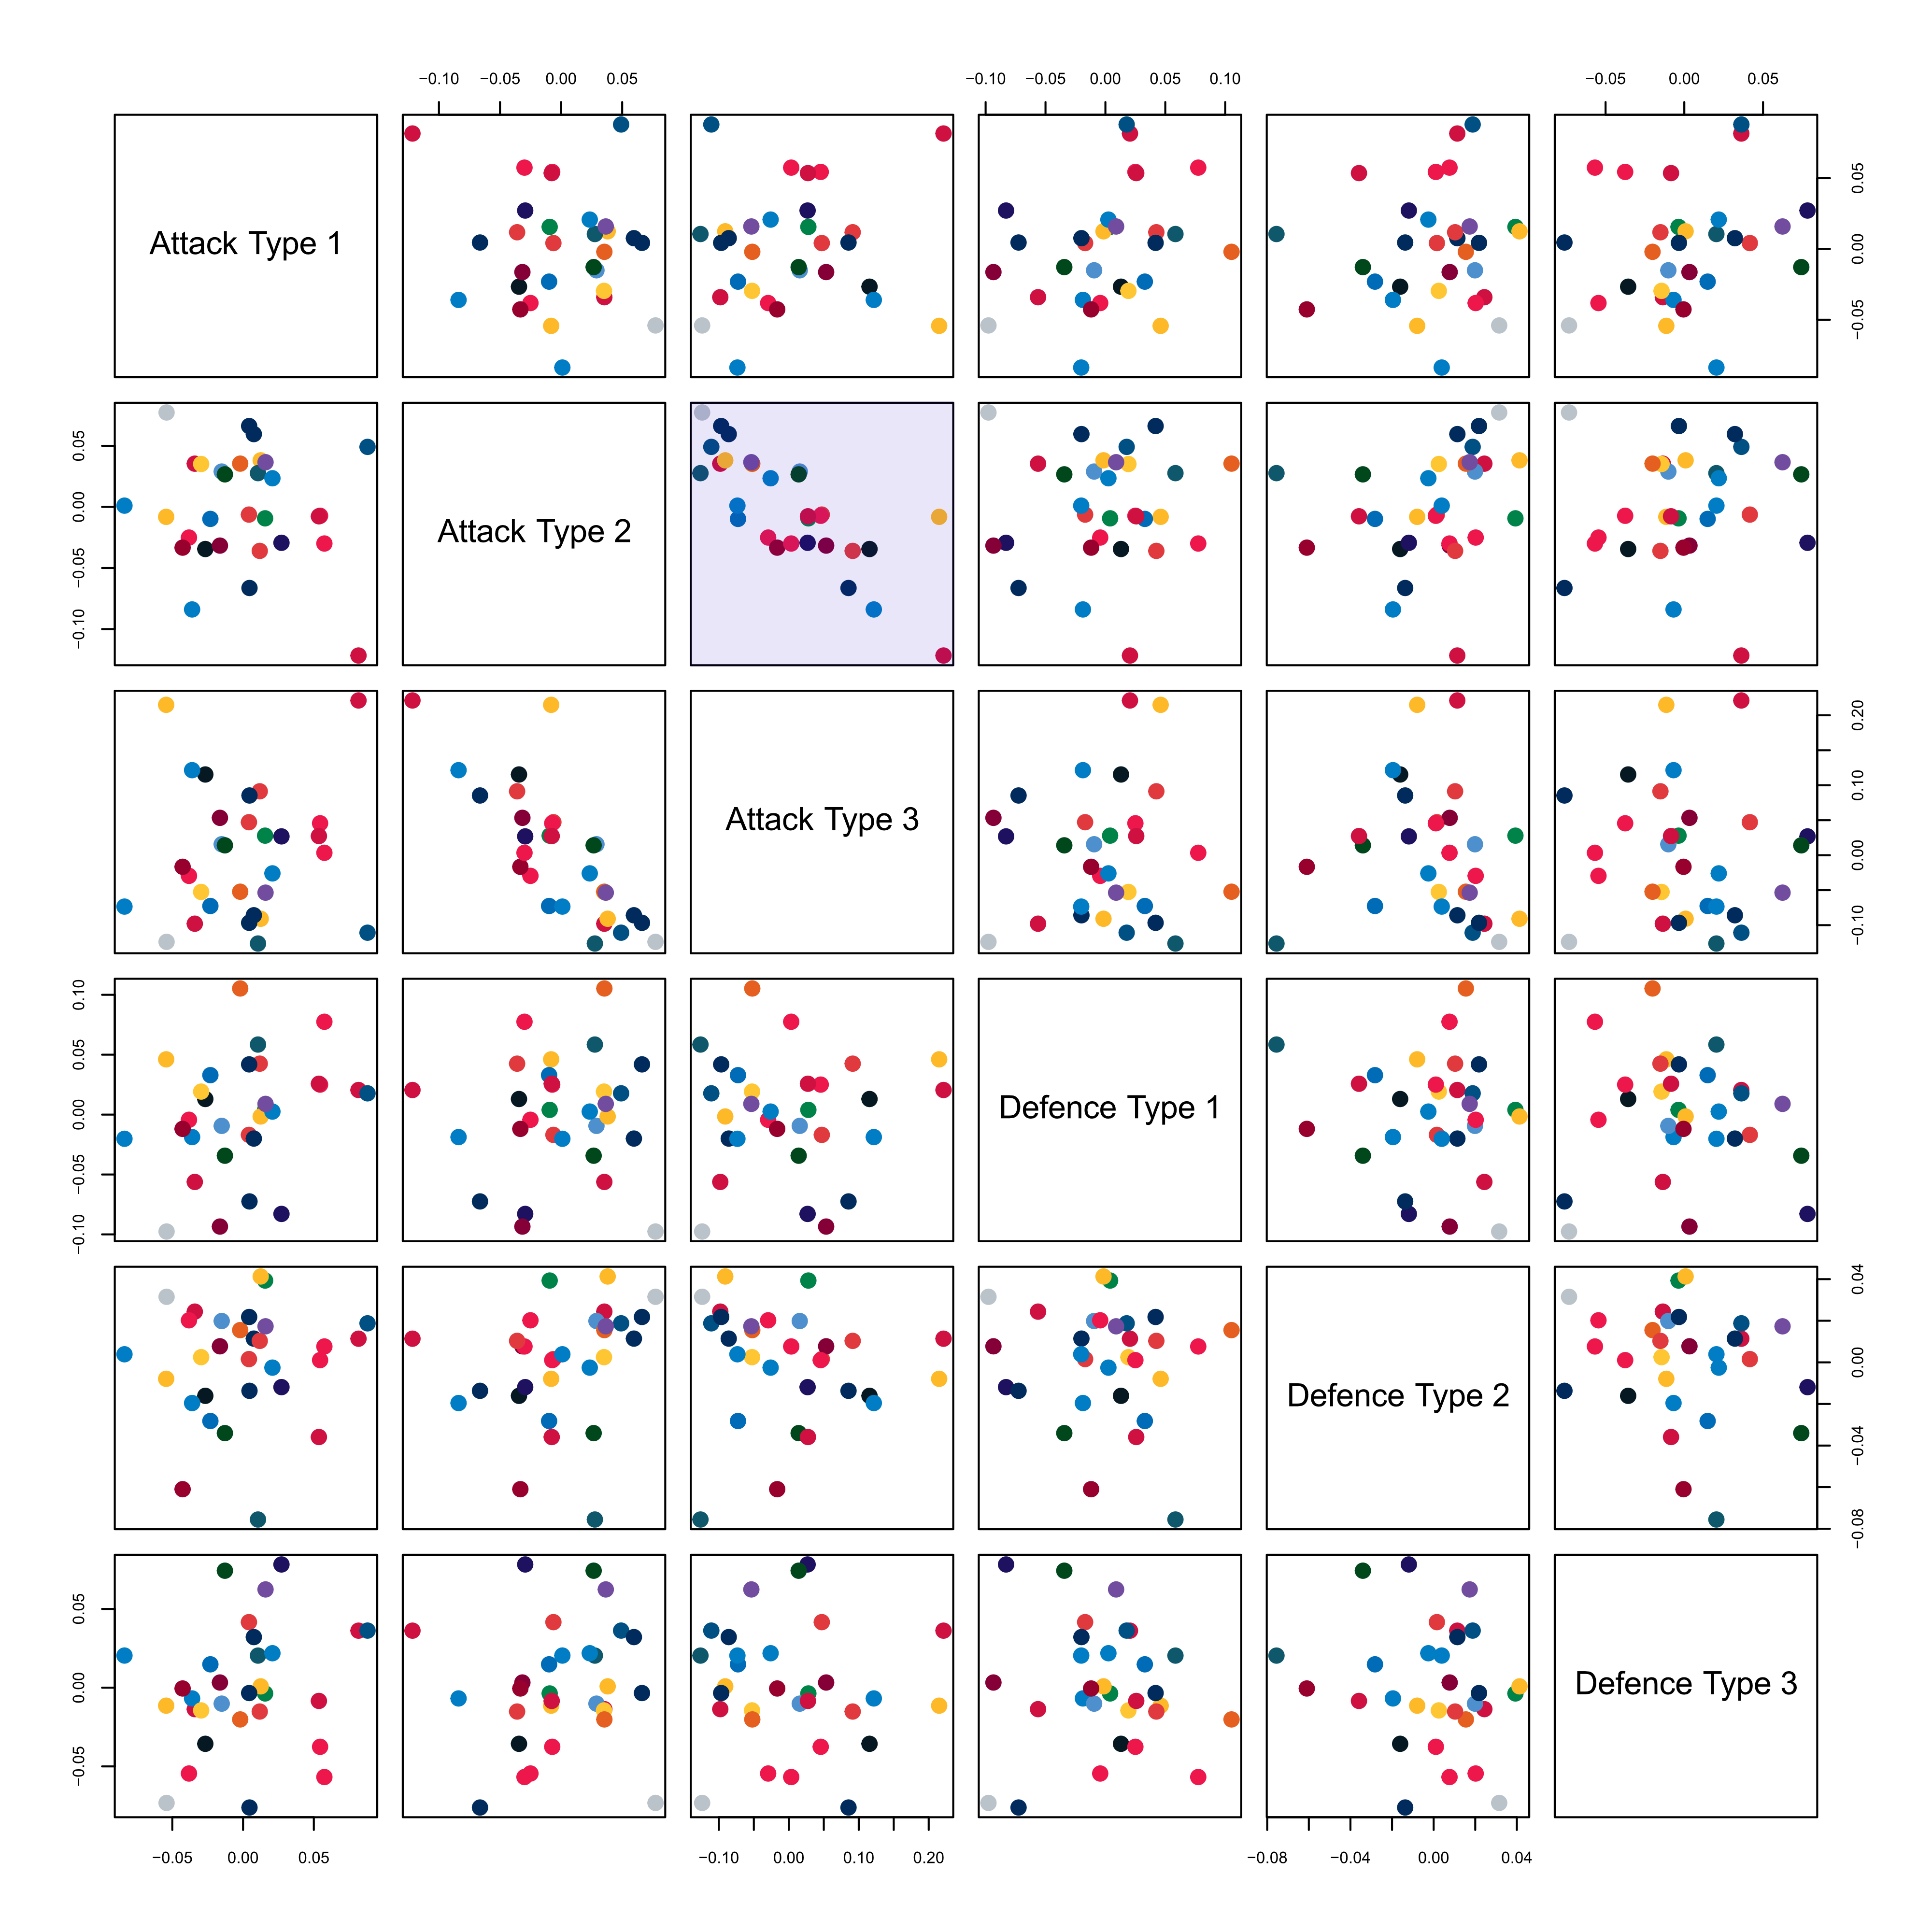
\includegraphics[width=1\textwidth]{Figures/Corr.png}
    \caption[Correlation]{Correlation between the different attacking and defending strengths}
    \label{fig:Corr}
\end{figure}

\noindent The correlation between attacking and defending strength for each scoring type can be seen in Figure \ref{fig:Corr}. From this figure we can see that there is a negative correlation between attacking strength of type 2 and 3 in the cell in row 2, column 3. This entails that teams who are very good at scoring with type 3 are bad at scoring or unwilling to score with type 2, and vice versa. The only team not following this norm is the Golden State Warriors, GSW. This makes sense because they have won 4 of the last 8 seasons excluding the 2019-2020 season, which means that they have been consistently good during these 8 seasons. There doesn't seem to be any correlation between attack and defence strengths, so the assumption that attack strength and defence strength are independent seem to mostly hold up looking at the correlation table.

\section{Strength of each team}

\noindent The attacking strengths for each team can be seen in Figure \ref{fig:Attack1}, \ref{fig:Attack2}, and \ref{fig:Attack3}, and the defending strengths can be seen in Figure \ref{fig:Defence1}, \ref{fig:Defence2}, and \ref{fig:Defence3}. Here we see which teams are the strongest at each scoring type. The expected values of the strength parameters are zero, so when a team has a strength of $0.10$, it is $e^{0.10} \approx 11\%$ stronger that the mean strength. This means that they will score $11\%$ more scores than a team with average strength. \\

\begin{table}[H]
\centering
\begin{tabular}{ |p{.5cm}|p{2cm}|p{2cm}|  }
    \hline
    $\text{k}$ & $\tau_{\text{A},\text{k}}^2$ & $\tau_{\text{D},\text{k}}^2$ \\
    \hline
    $1$ & $0.0016857$ & $0.0023295$ \\
    $2$ & $0.0020435$ & $0.0007715$ \\
    $3$ & $0.0084381$ & $0.0016362$ \\
    \hline
\end{tabular}
\caption{Variances of the Random Effects}
\label{table:randomEffCovidVar}
\end{table}

\noindent The variances for the random effects can be seen in Table \ref{table:randomEffCovidVar}. From this table we can see that the three points attacking strength vary much more than the other attacking types and all defending types. This makes sense because the three point shot is the hardest scoring type, so all teams cannot be equally as good with that type. Also the two-pointers don't vary as much, which means that all teams score almost the same amount of two-pointers.

\begin{figure}[H]
    \centering
    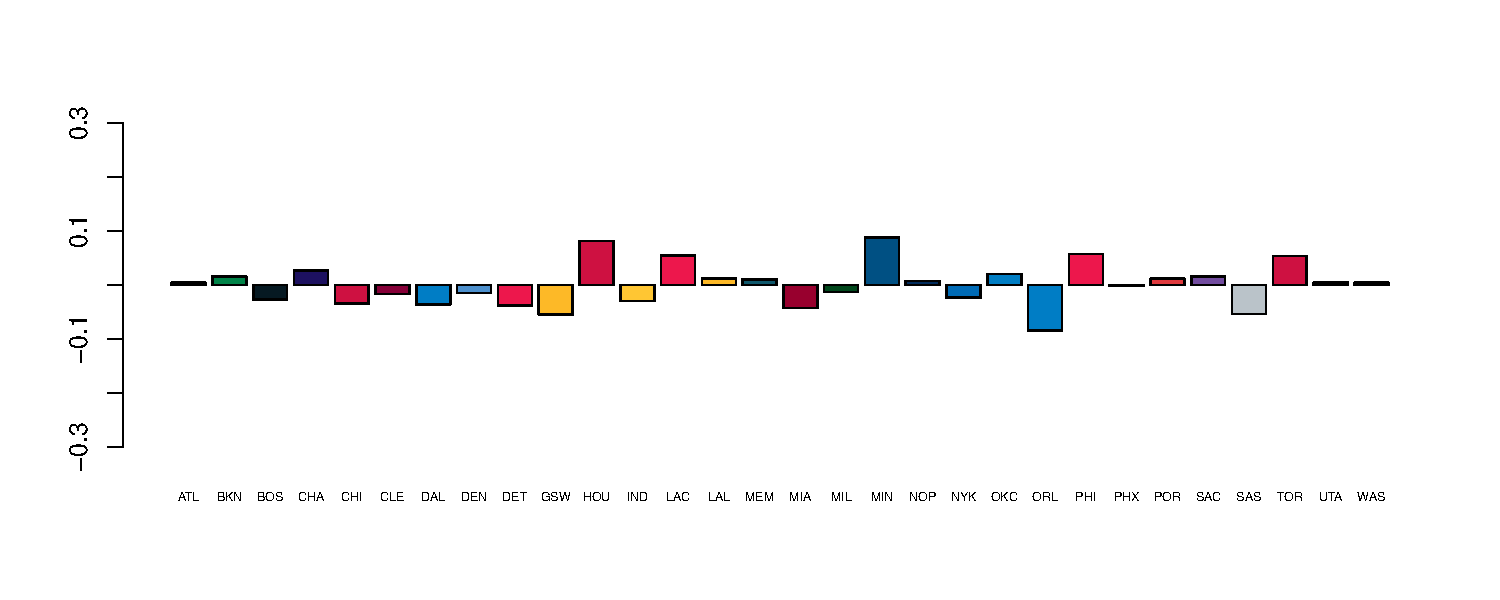
\includegraphics[width=1\textwidth]{Figures/Attack1.pdf}
    \caption[Attack1]{Strength of attacking type 1.}
    \label{fig:Attack1}
\end{figure}

\begin{figure}[H]
    \centering
    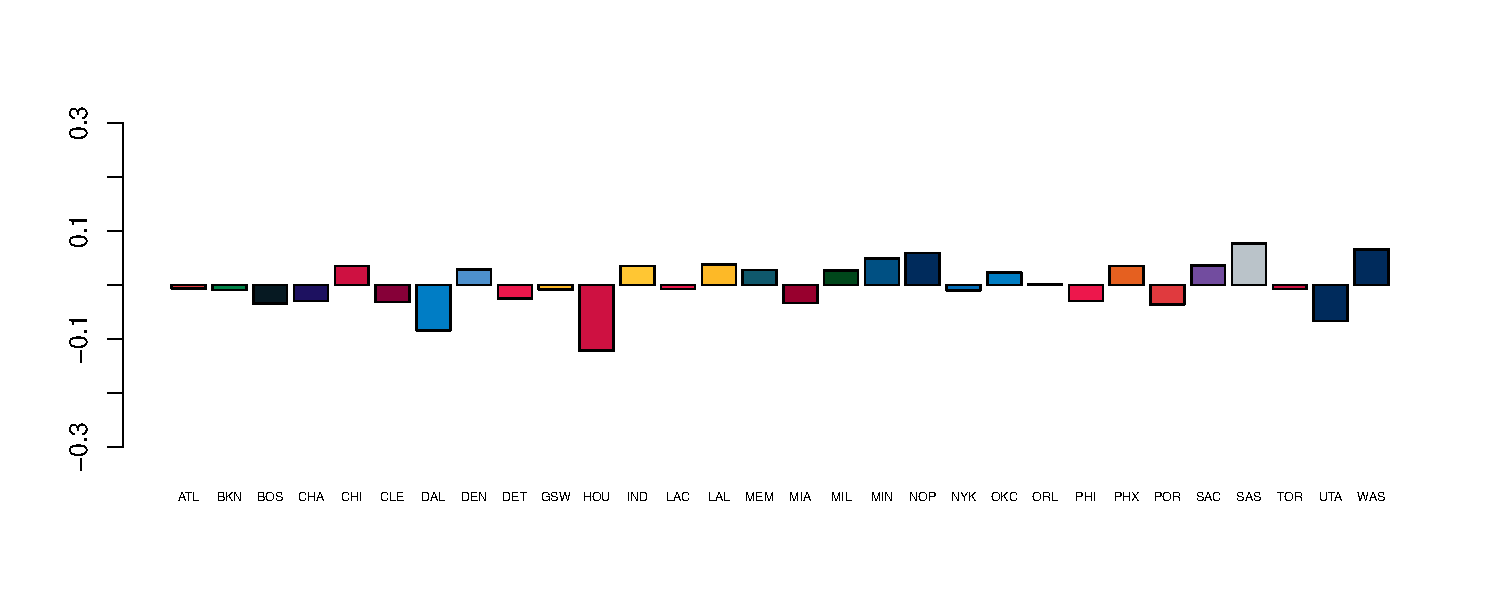
\includegraphics[width=1\textwidth]{Figures/Attack2.pdf}
    \caption[Attack2]{Strength of attacking type 2.}
    \label{fig:Attack2}
\end{figure}


\begin{figure}[H]
    \centering
    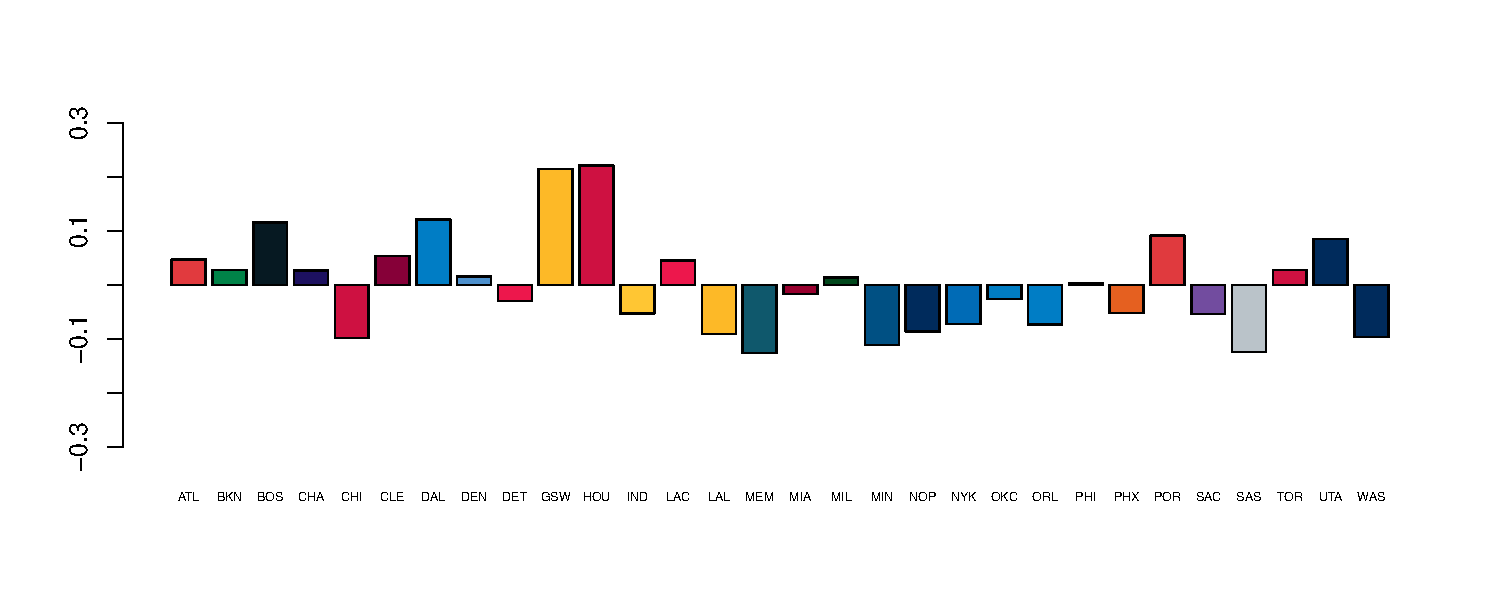
\includegraphics[width=1\textwidth]{Figures/Attack3.pdf}
    \caption[Attack3]{Strength of attacking type 3.}
    \label{fig:Attack3}
\end{figure}

\begin{figure}[H]
    \centering
    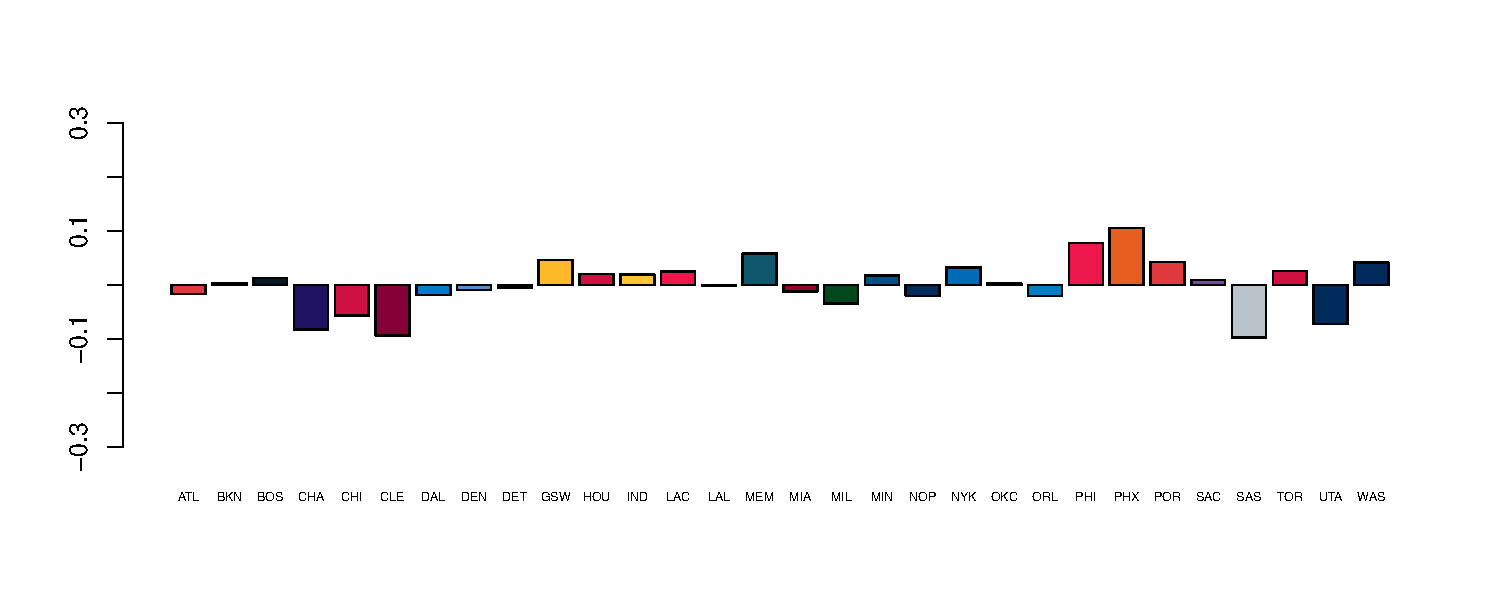
\includegraphics[width=1\textwidth]{Figures/Defence1.pdf}
    \caption[Attack1]{Strength of defending type 1.}
    \label{fig:Defence1}
\end{figure}

\begin{figure}[H]
    \centering
    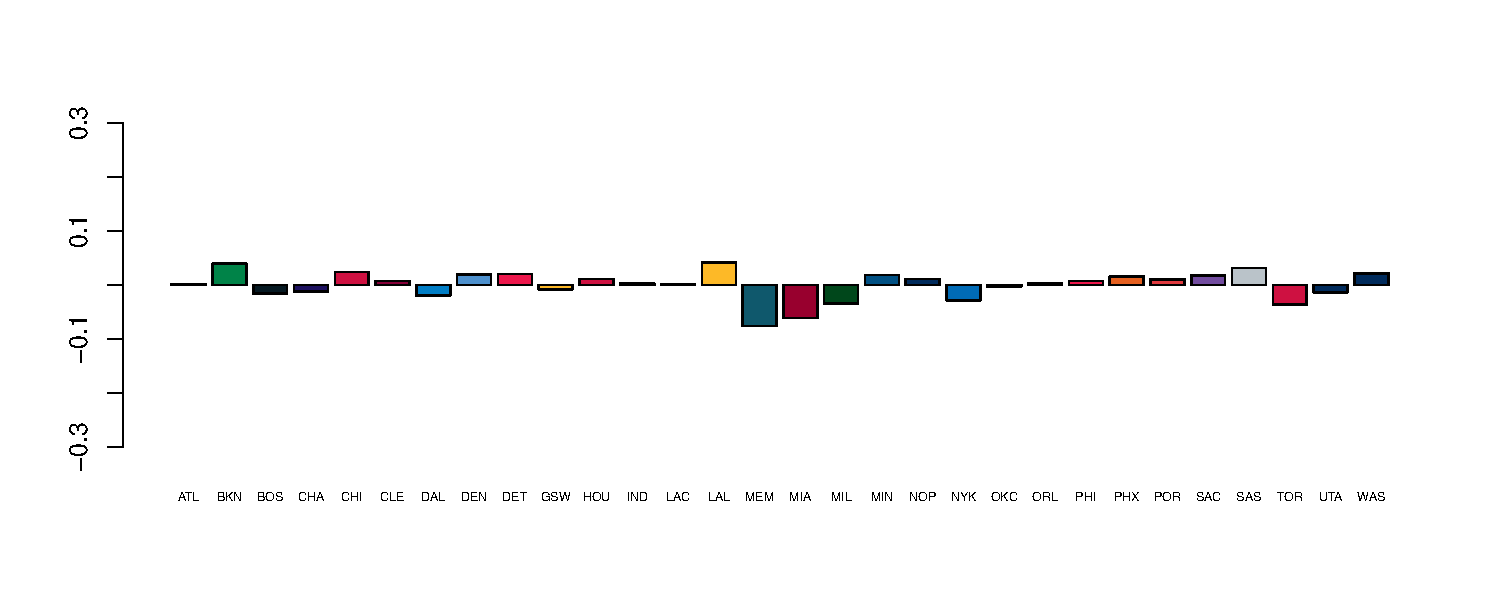
\includegraphics[width=1\textwidth]{Figures/Defence2.pdf}
    \caption[Attack2]{Strength of defending type 2.}
    \label{fig:Defence2}
\end{figure}

\begin{figure}[H]
    \centering
    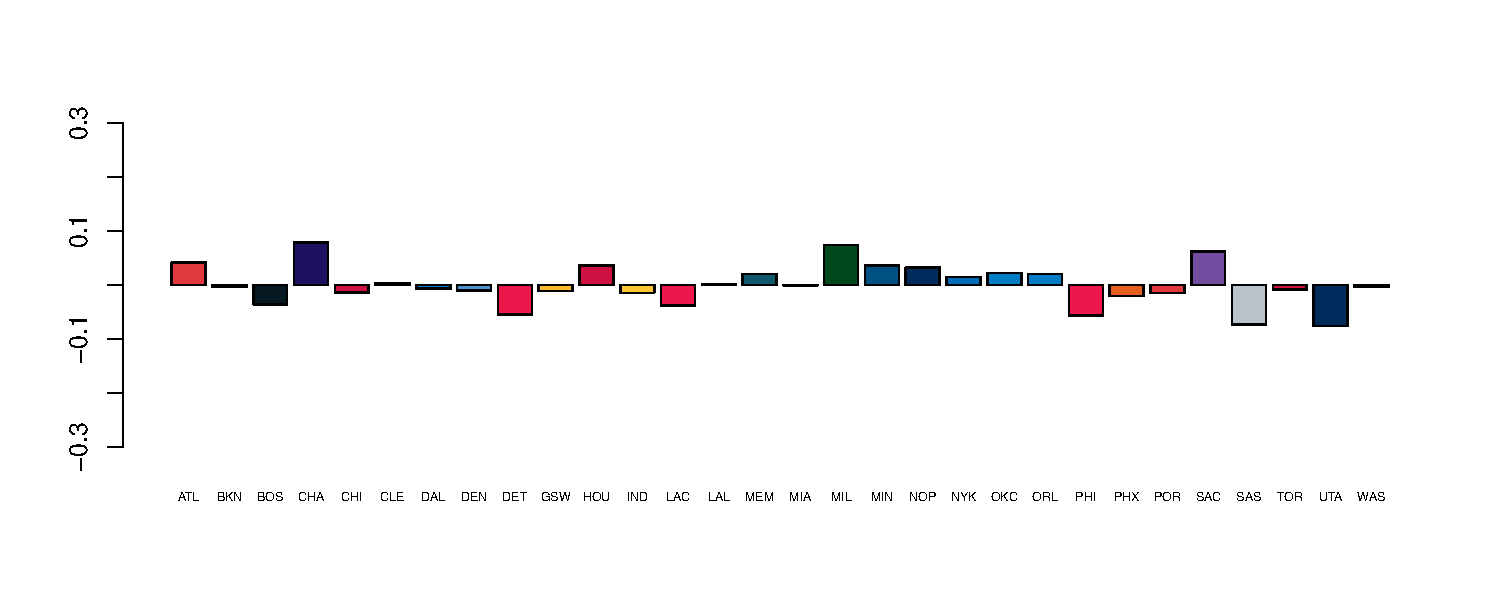
\includegraphics[width=1\textwidth]{Figures/Defence3.pdf}
    \caption[Attack3]{Strength of defending type 3.}
    \label{fig:Defence3}
\end{figure}

\section{Covid-19 impact and home court advantage}

\noindent From Table \ref{table:fixedEffExpCovid} we can see the influence that the home court had and that Covid had on every scoring type. In the last column, we can also see that during covid, the homecourt advantage got $1.23\%$ smaller during covid. There could be many reasons why the homecourt advantage got smaller, but one explanation of this could be that there were no fans spectating, and with less fans the home team didn't get the same boost that a full arena would give them. \\

\section{Number of fans}

\noindent Another interesting influence on the number of scores could be the number of fans spectating. The best model for this is,

\begin{equation}
\begin{aligned}
    \log(\lambda_{i,j,\text{k}}) &= \beta_\text{k} + \beta_{\text{H},\text{k}} \ x_\text{H,ij\text{k}} + \beta_{\text{FANS},\text{k}} \ x_\text{FANS,ij\text{k}} \\
    &+ \beta_\text{H.FANS} \ x_\text{H.FANS,ij\text{k}} + \gamma_{\text{A},i,\text{k}} + \gamma_{\text{D},j,\text{k}},
\label{eq:bestmodelfans}
\end{aligned}
\end{equation}

\noindent which I found using the same method for testing as in Section \ref{modsel}. This model is almost identical to the model in Equation \ref{eq:bestmodelcovid} but instead of Covid we are using the number of fans present at a match. $x_\text{FANS}$ and $x_\text{H.FANS}$ is then the number of fans present in a normal match and a normal match at home respectively. When the number of fans at a match is zero, this model is essentially the same as the model in Equation \ref{eq:bestmodelcovid} during covid. Table \ref{table:fixedEffExpFans} show the influence that a single fan has and the influence $20.000$ fans has on the total amount of scores of each type. The last column show the influence added when having home court advantage. This table also show the amount of points during covid, because there were no fans present. It suggest that when the number of fans increased, the total amount of one-pointers and two-pointers increased but the total amount of three-pointers decreased. This is because during covid, the total amount of three-pointers scored in a match increased, as shown in Table \ref{table:fixedEffExpCovid}.

\begin{table}[!ht]
\centering
\begin{tabular}{ |p{.5cm}|p{2cm}|p{3cm}|p{2cm}|p{2cm}| }
    \hline
    $\text{k}$ & $e^{\hat\beta_\text{k}}$ & $e^{\hat\beta_{\text{FANS},\text{k}}}$ & $e^{\hat\beta_{\text{FANS},\text{k}} \cdot 20000}$ & $\beta_\text{H.FANS}$ \\
    \hline
    $1$ & $\approx 17$ & $\approx 0.0001\%$ & $\approx 2.1\%$ & $\approx 0.0001\%$ \\
    $2$ & $\approx 28$ & $\approx 0.0001\%$ & $\approx 2.5\%$ & $\approx 0.0001\%$ \\
    $3$ & $\approx 13$ & $\approx -0.0012\%$ & $\approx -20.7\%$ & $\approx 0.0001\%$ \\
    \hline
\end{tabular}
\caption{Exponential value of the Fixed Effects using the model with fans}
\label{table:fixedEffExpFans}
\end{table}

\newpage

\section{Extension of the best model}

\noindent This thesis has only used the strength of a team according to 8 seasons worth of data, but because some teams change a lot inbetween and during seasons, a more interesting approach could be to use the AR(1) process to find the strengths of each team where they changes during the seasons. This could tell us if some teams tend to be stronger at the start, middle or end of a season, and how their strengths have changed throughout the years. But since there are some breaks in a season, one could maybe use the OU process to find the strengths during a season. The OU process can account for irregularities of the times where values are recorded, and can therefore be more useful. This new OU model has the same formula as the best model in section \ref{bestmod}, but the random effects are now modelled as a OU process. Tables \ref{table:fixedEffCovidOU} and \ref{table:fixedEffExpCovidOU} show the fixed effects and the exponential of the fixed effects respectively. These tables are pretty similar to tables \ref{table:fixedEffCovid} and \ref{table:fixedEffExpCovid}, but the covid term now give a positive impact on one- and two-poiners. This may be because now the attacking strengths of each team are not constant, but changes over time, so their strengths during covid could be slightly lower to account for this. This can be seen in Figures \ref{fig:OU1}, \ref{fig:OU2}, and \ref{fig:OU3} where the highlighted areas are the covid season. From Figure \ref{fig:OU3} we can see that the attacking strengths have increased a lot throughout the years for every team. Figures \ref{fig:GSW_2_OU}, \ref{fig:GSW_3_OU}, \ref{fig:HOU_2_OU}, and \ref{fig:HOU_3_OU} show the attacking strengths of the Golden State Warriors and Houston Rockets for both two-pointers and three-pointers. These two teams had the best three-points strengths, so it will be interesting to see how they compare throughout the years. We see that GSW has been very consistent with their strengths except for their two-pointer strength in the later seasons, but HOU have been very bad with two-pointers and inconsistent with three-pointers. This is due to them losing the players who scored three-pointers for them and GSW has kept most of theirs.

\begin{table}[!ht]
\centering
\begin{tabular}{ |p{.3cm}|p{3cm}|p{3cm}|p{3cm}|p{3cm}|  }
    \hline
    $\text{k}$ & $\hat\beta_\text{k} \pm SD(\hat\beta_\text{k})$& $\hat\beta_{\text{H},\text{k}} \pm SD(\hat\beta_{\text{H},\text{k}})$ & $\hat\beta_{\text{C},\text{k}} \pm SD(\hat\beta_{\text{C},\text{k}})$ & $\hat\beta_\text{HC} \pm SD(\hat\beta_\text{HC})$ \\
    \hline
    $1$ & $2.8298 \pm 0.0148$ & $0.0339 \pm 0.0035$ & $0.0387 \pm 0.0230$ & $-0.0126 \pm 0.0061$ \\
    $2$ & $3.3645 \pm 0.0147$ & $0.0167 \pm 0.0028$ & $0.0158 \pm 0.0224$ & $-0.0126 \pm 0.0061$ \\
    $3$ & $2.3134 \pm 0.0150$ & $0.0278 \pm 0.0045$ & $0.0926 \pm 0.0240$ & $-0.0126 \pm 0.0061$ \\
    \hline
\end{tabular}
\caption{Fixed Effects $\pm$ Standard Deviations for the OU model}
\label{table:fixedEffCovidOU}
\end{table}

\begin{table}[!ht]
\centering
\begin{tabular}{ |p{.5cm}|p{2cm}|p{2cm}|p{2cm}|p{2cm}|  }
    \hline
    $\text{k}$ & $e^{\hat\beta_\text{k}}$ & $e^{\hat\beta_{\text{H},\text{k}}}$ & $e^{\hat\beta_{\text{C},\text{k}}}$ & $e^{\hat\beta_\text{HC}}$ \\
    \hline
    $1$ & $\approx 17$ & $\approx 3.45\%$ & $\approx 3.95\%$ & $\approx -1.25\%$ \\
    $2$ & $\approx 29$ & $\approx 1.68\%$ & $\approx 1.59\%$ & $\approx -1.25\%$ \\
    $3$ & $\approx 10$ & $\approx 2.81\%$ & $\approx 9.70\%$ & $\approx -1.25\%$ \\
    \hline
\end{tabular}
\caption{Exponential value of the Fixed Effects for the OU model}
\label{table:fixedEffExpCovidOU}
\end{table}

\begin{figure}[H]
    \centering
    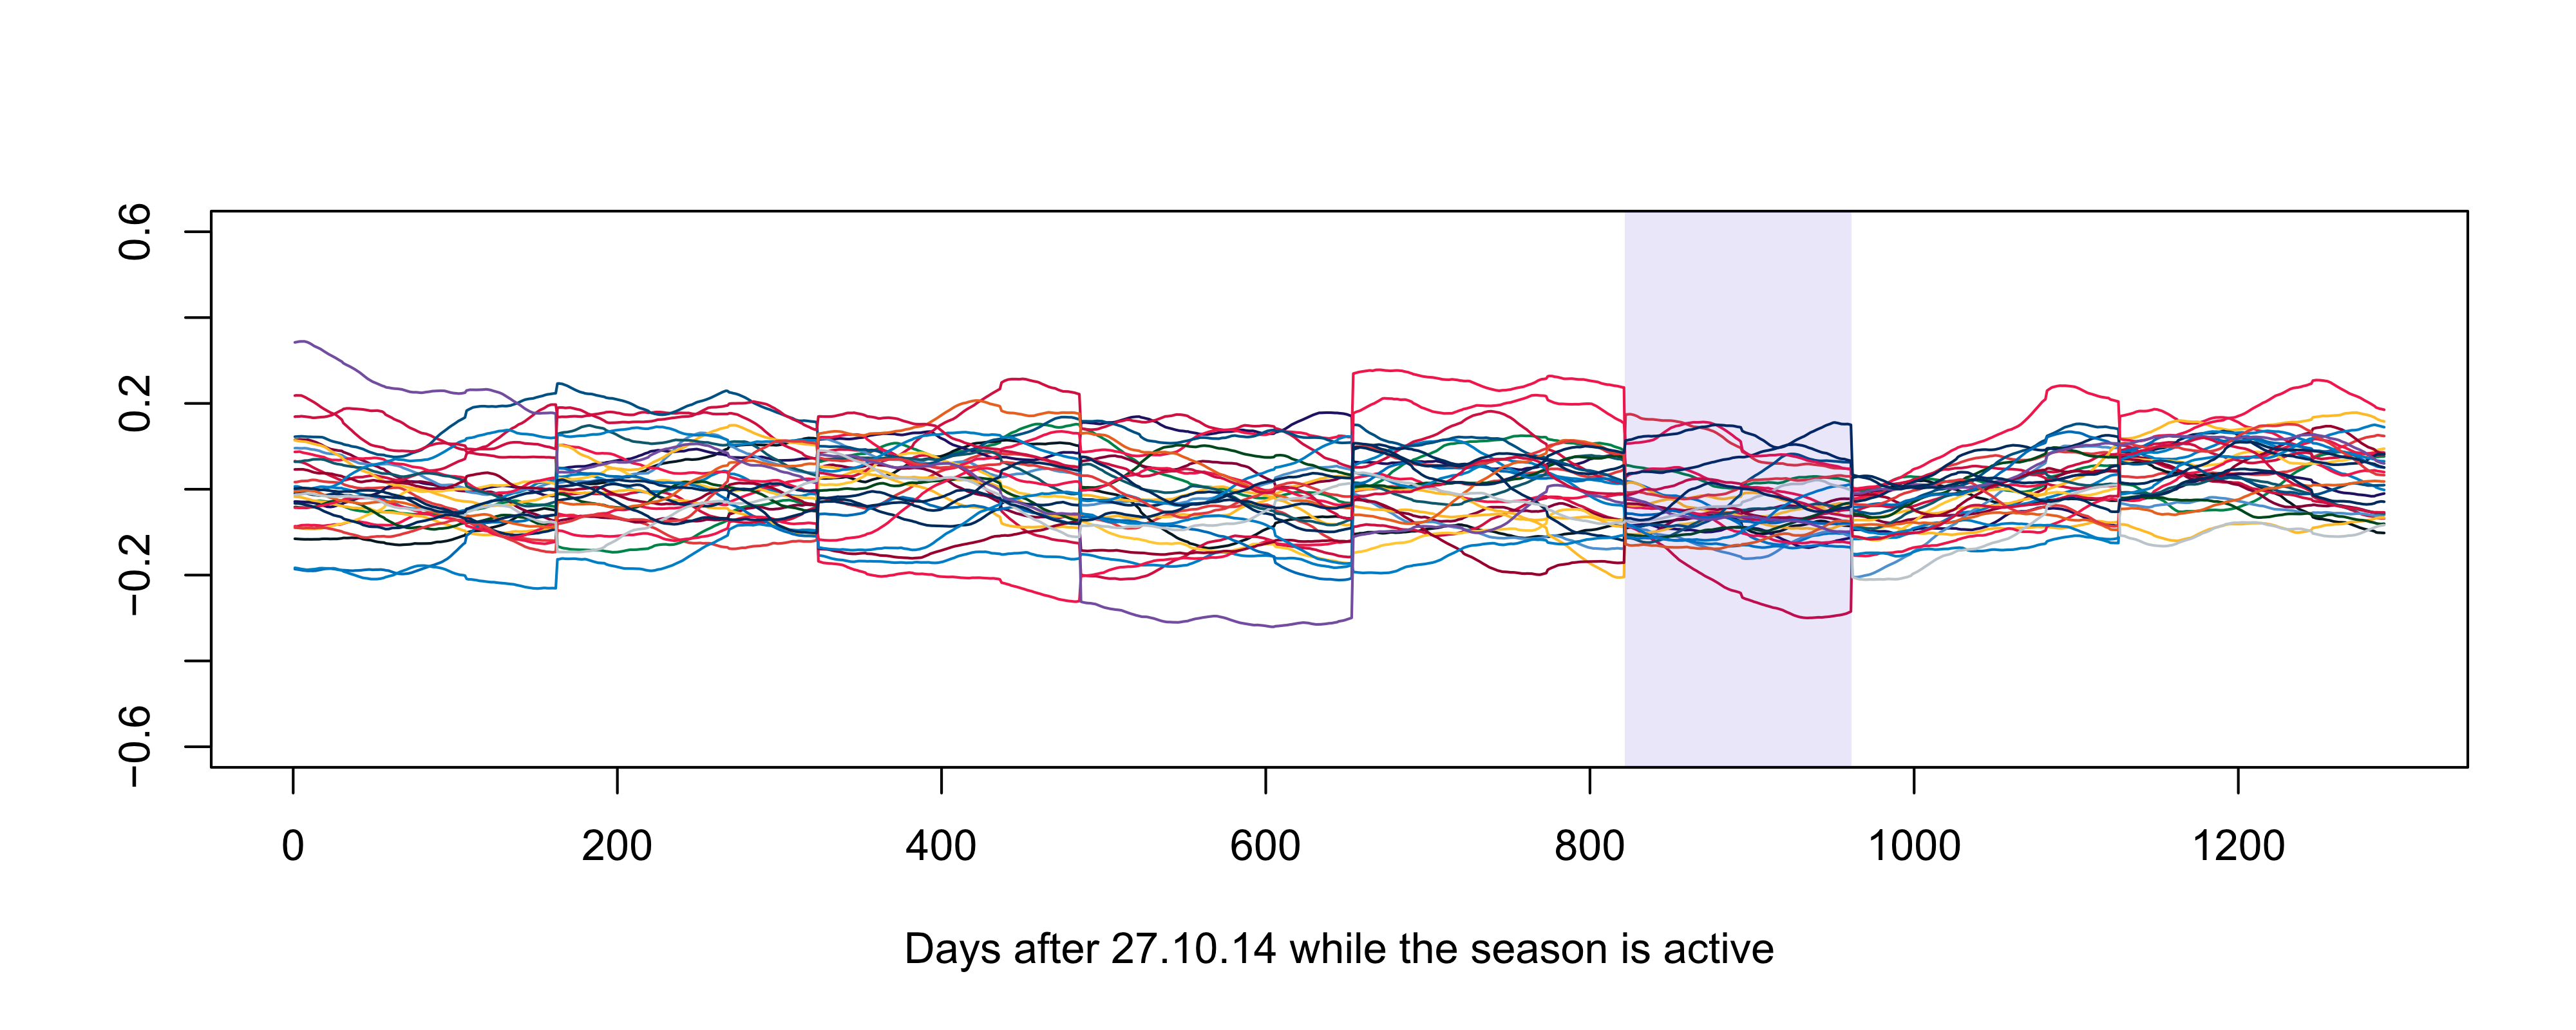
\includegraphics[width=1\textwidth]{Figures/OU1.png}
    \caption[OU1]{Strength of attacking type 1 using the OU model where the highlighted area is the covid season}
    \label{fig:OU1}
\end{figure}

\begin{figure}[H]
    \centering
    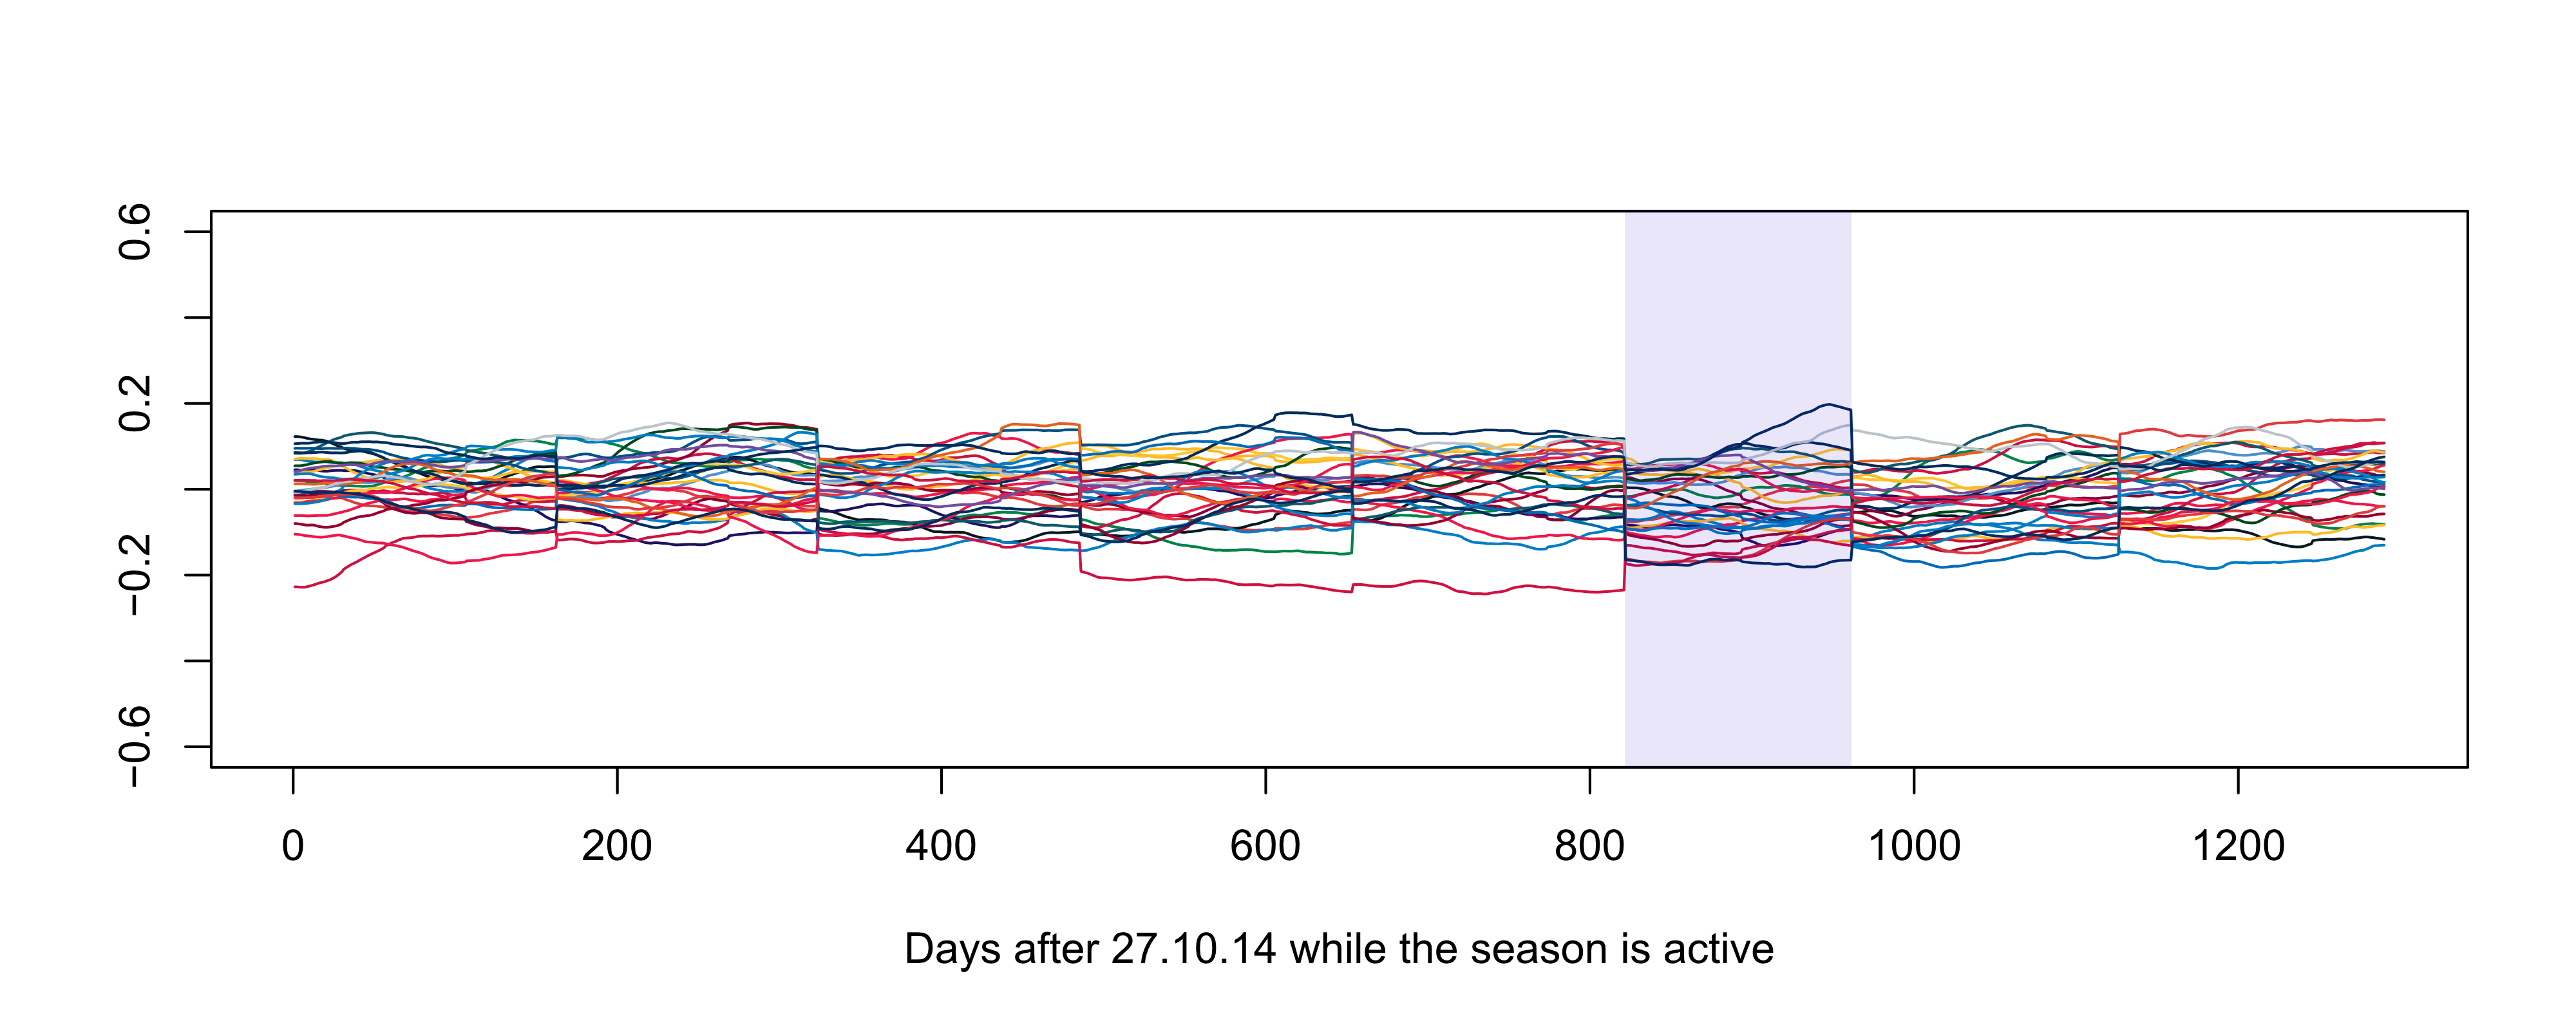
\includegraphics[width=1\textwidth]{Figures/OU2.png}
    \caption[OU2]{Strength of attacking type 2 using the OU model where the highlighted area is the covid season}
    \label{fig:OU2}
\end{figure}

\begin{figure}[H]
    \centering
    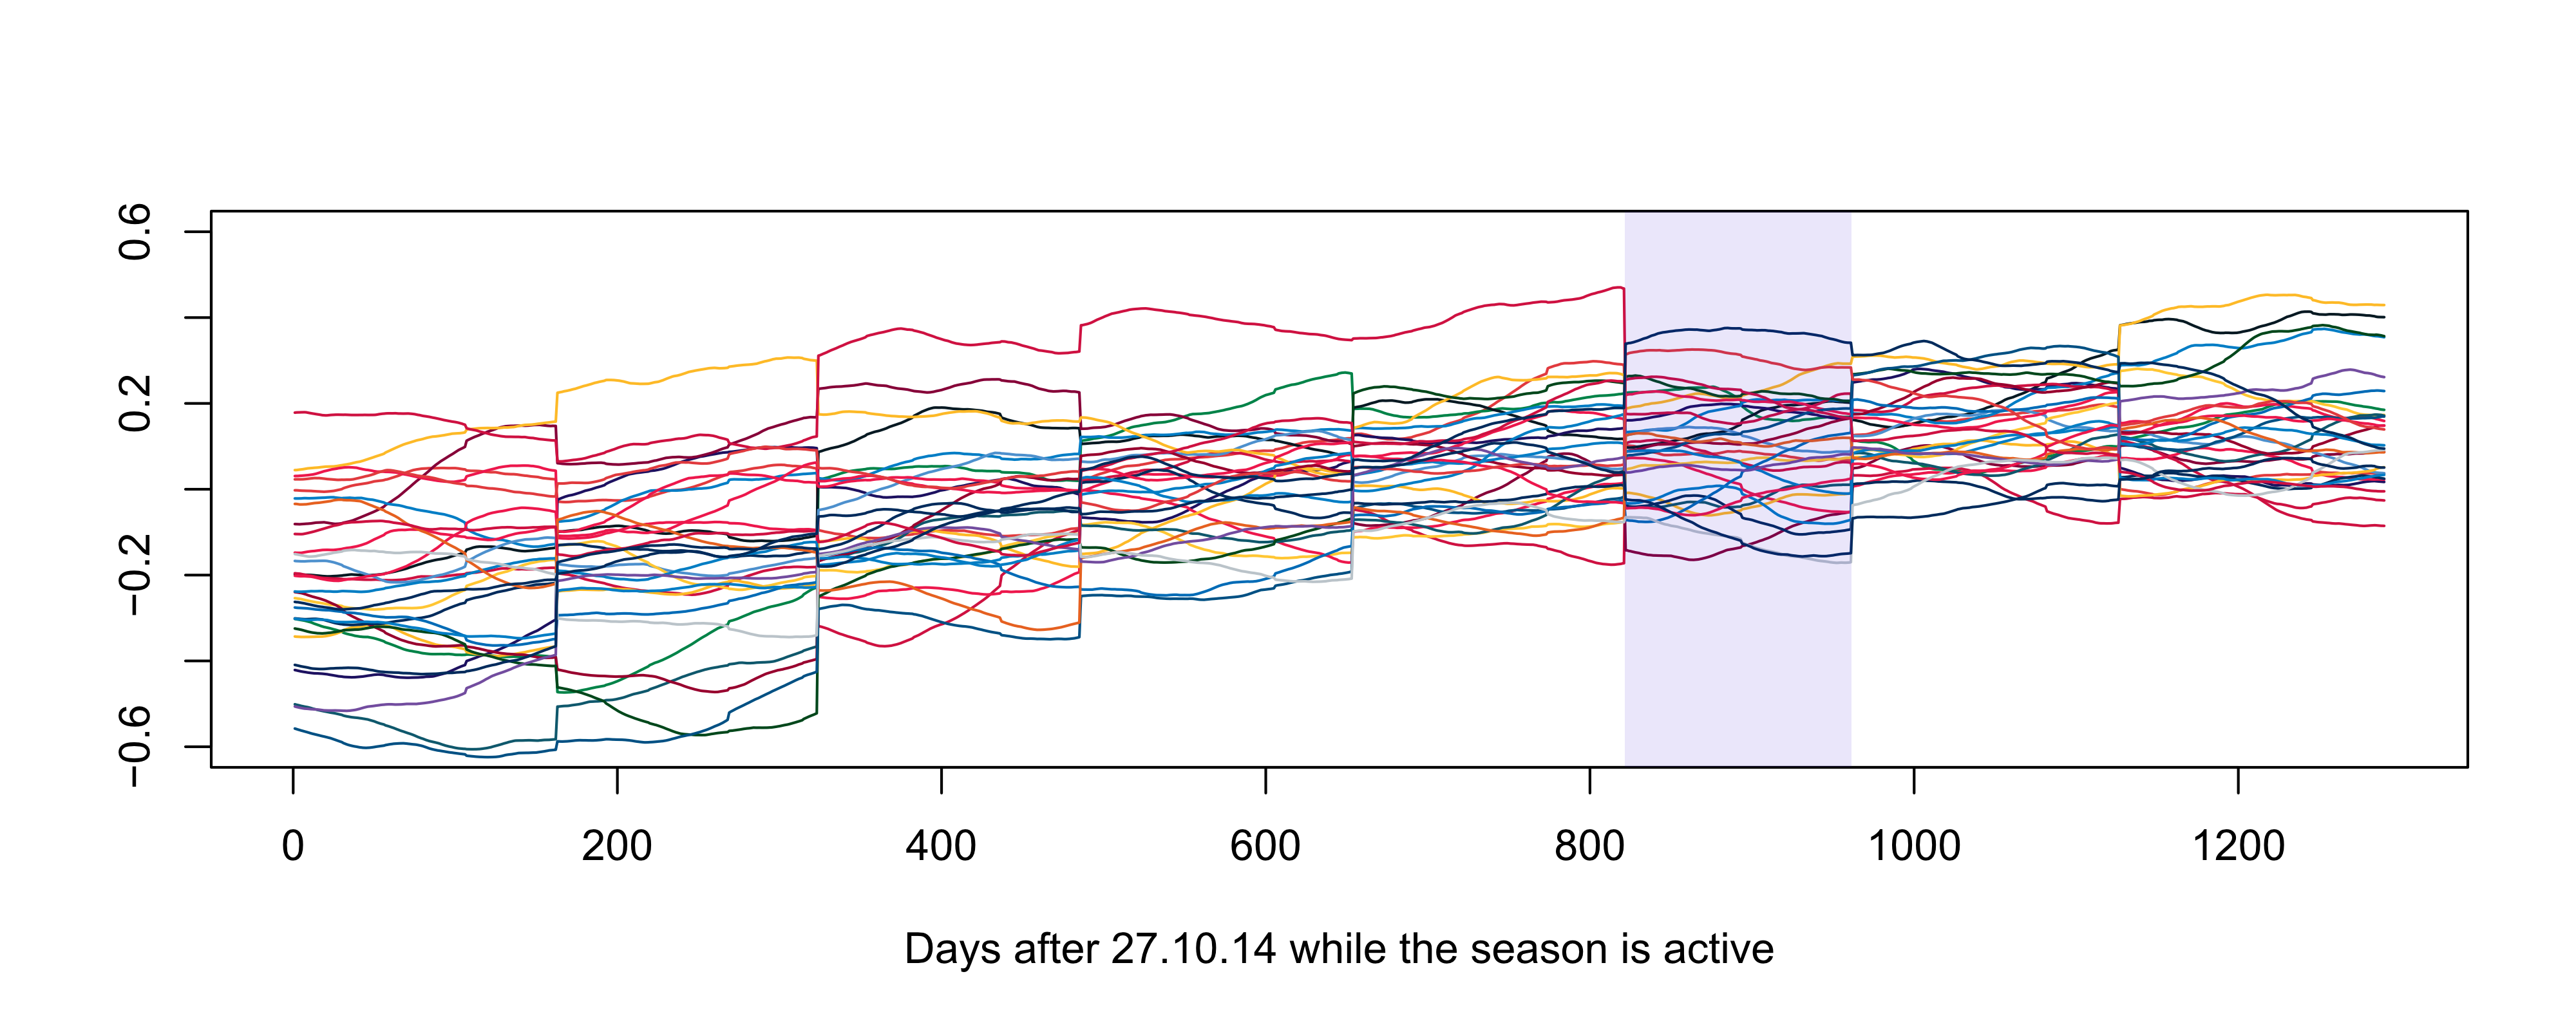
\includegraphics[width=1\textwidth]{Figures/OU3.png}
    \caption[OU3]{Strength of attacking type 3 using the OU model where the highlighted area is the covid season}
    \label{fig:OU3}
\end{figure}

\begin{figure}[H]
    \centering
    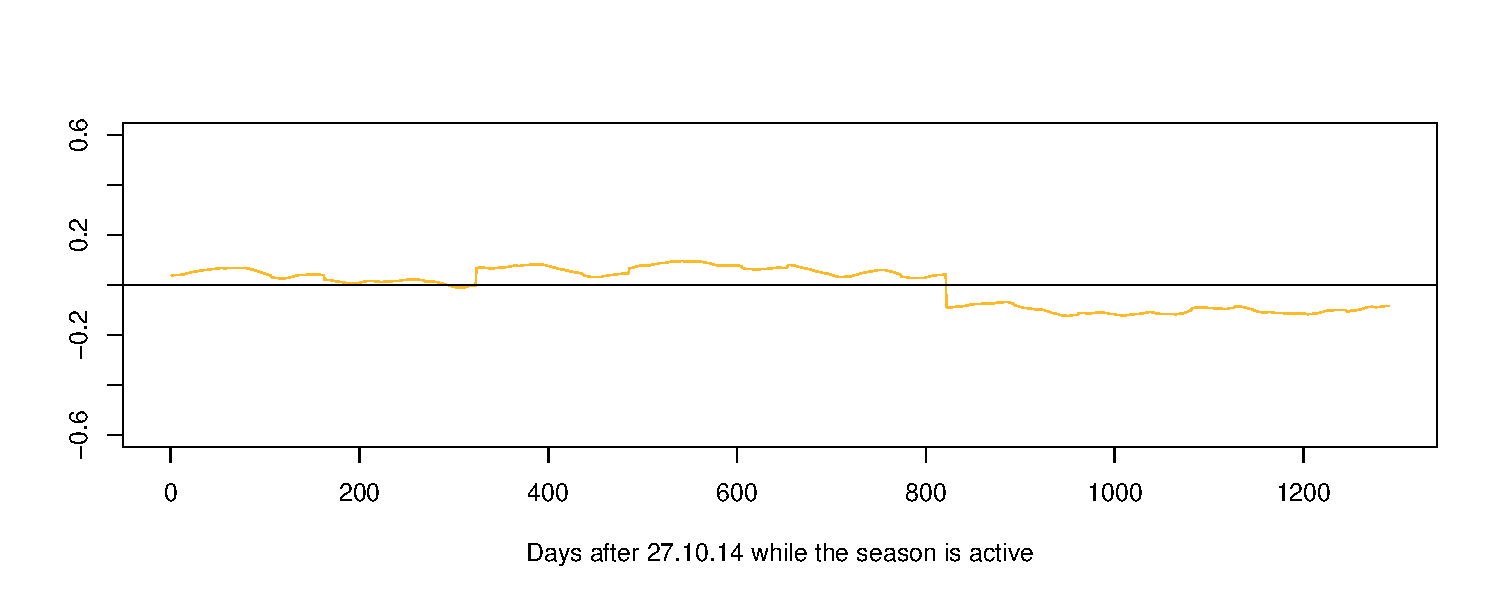
\includegraphics[width=.8\textwidth]{Figures/GSWOU2.pdf}
    \caption[GSW2OU]{GSW Attack strength type 2}
    \label{fig:GSW_2_OU}
\end{figure}

\begin{figure}[H]
    \centering
    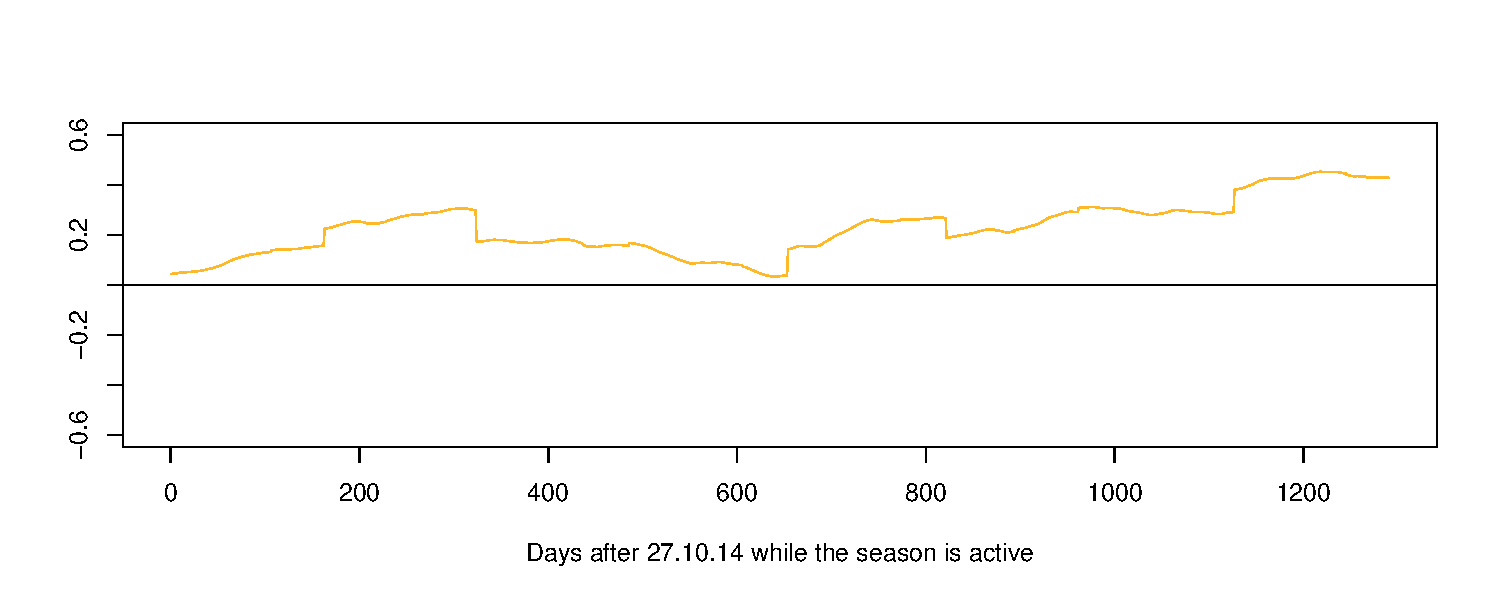
\includegraphics[width=.8\textwidth]{Figures/GSWOU3.pdf}
    \caption[GSW3OU]{GSW Attack strength type 3}
    \label{fig:GSW_3_OU}
\end{figure}

\begin{figure}[H]
    \centering
    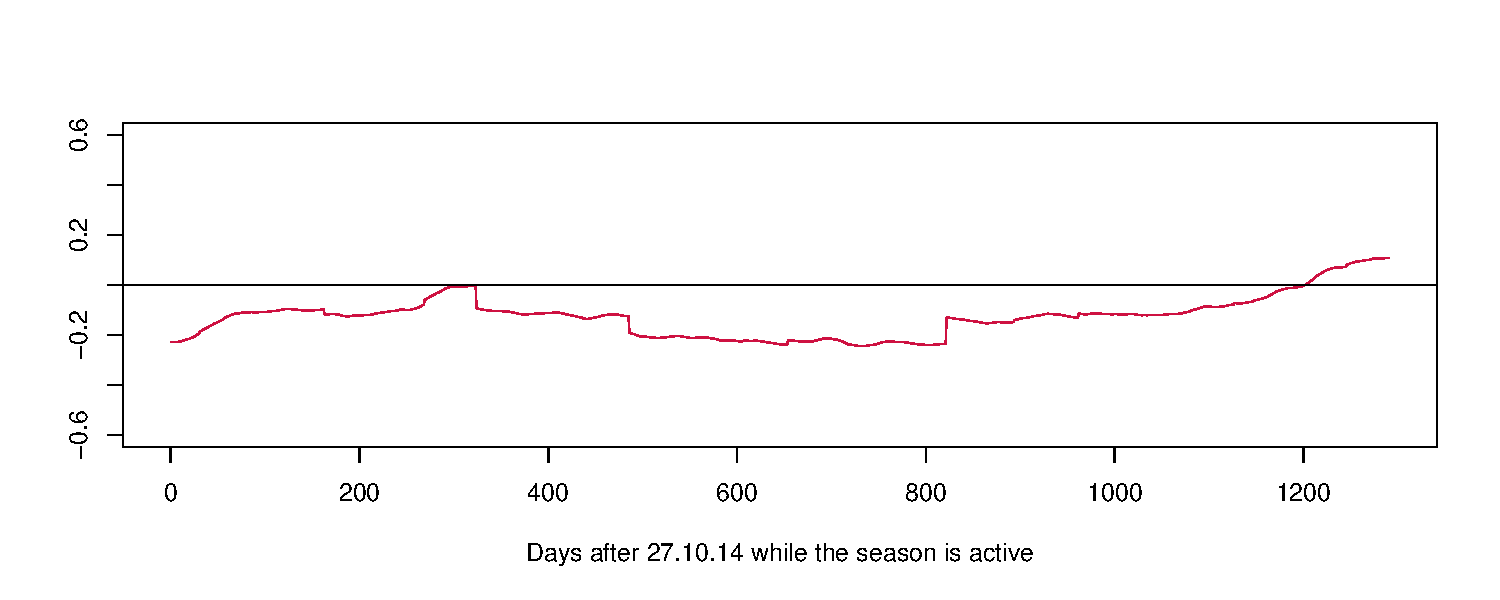
\includegraphics[width=.8\textwidth]{Figures/HOUOU2.pdf}
    \caption[HOU2OU]{HOU Attack strength type 2}
    \label{fig:HOU_2_OU}
\end{figure}

\begin{figure}[H]
    \centering
    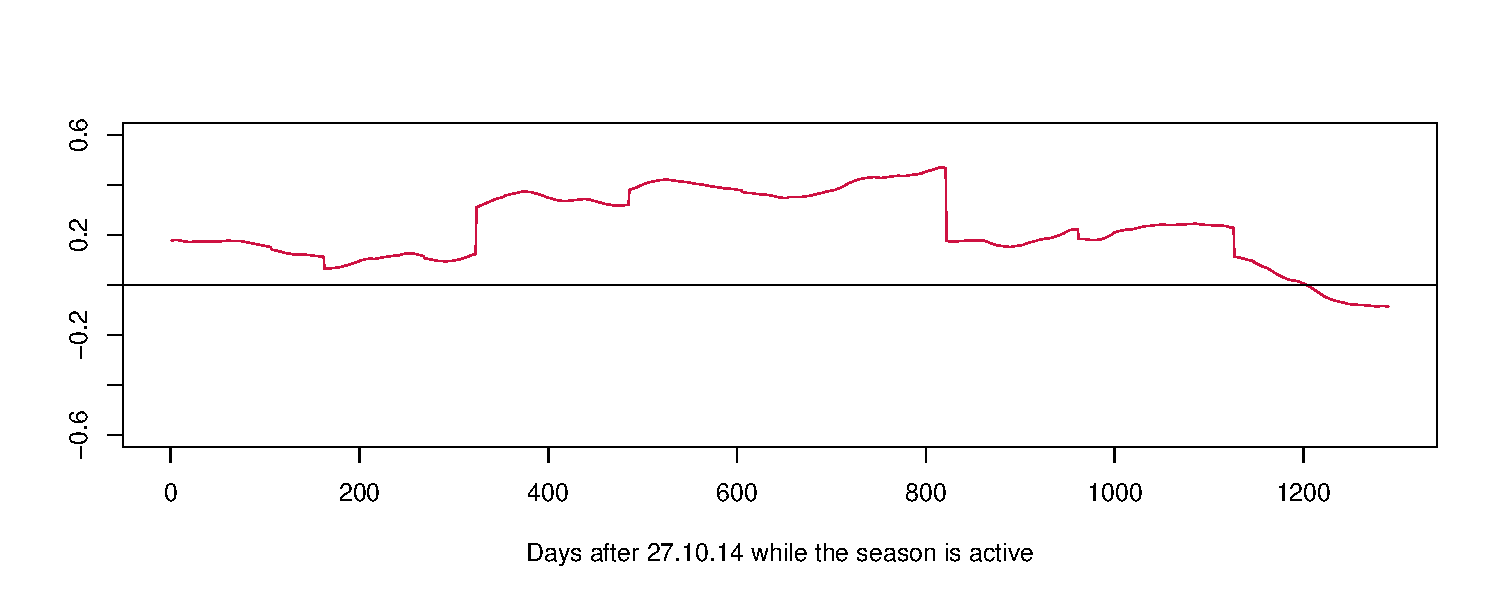
\includegraphics[width=.8\textwidth]{Figures/HOUOU3.pdf}
    \caption[HOU3OU]{HOU Attack strength type 3}
    \label{fig:HOU_3_OU}
\end{figure}

\newpage

\section{Future work}  \label{future}

\noindent The variance of the number of fouls committed in a match is difficult to account for, because it is random, but in close matches there are an overabundance of fouls committed in an attempt to catch up to the opponent, which is closer looked at in \cite{poissonNBA}. To show that there is overdispersion for this in the data, I will first assume that the number of fouls committed, $X$ in a match is Poisson distributed with rate $\lambda$, I will also assume that the number of scores, $Y$, conditional on the number of fouls is binomially distributed with parameters $2X$ and $p$, where we have an average of 2 attempts per foul. I.e.,

\begin{equation}
    X \sim Poisson(\lambda),
\end{equation}

\begin{equation}
    Y|X=x \sim Bin(2X,p).
\end{equation}

\noindent For finding the marginal expectation and variance of $Y$, I will use the law of total expectation and law of total variance.

\begin{equation}
\begin{aligned}
    E[Y] &= E[E[Y|X]] \\
        &= E[2Xp] \\
        &= 2\lambda p
\end{aligned}
\end{equation}

\begin{equation}
\begin{aligned}
    Var[Y] &= E[Var[Y|X]] + Var[E[Y|X]] \\
        &= E[2Xp(1-p)] + Var[2Xp] \\
        &= 2\lambda p(1-p) + 4p^2\lambda \\
        &= E[y](1-p + 2p) \\
        &= E[y](1 + p) \\
\end{aligned}
\end{equation}

\noindent Since $(1 + p)$ is larger than one, this underlying data-generating process would generate overdispersion in the data.

\cleardoublepage


\chapter{Conclusions}

\noindent In conclusion, the differences between the covid season and the other seasons analyzed is that the home-court advantage got smaller, but it did not disappear fully. This could be that because they still played near were they lived, so they still got a boost. Where that boost could come from could differ from player to player, but the main boost could come from better sleep or better relaxation before a match. This is because they were still in their home city. Also the number of fans at a match had a positive impact on all scoring types except three-pointers and they had a positive impact on the home-court advantage. The impact an individual fan had on the home-court advantage was positive in all three scoring types, but they had a negative impact on the number of three-pointers scored. This is because during covid, they scored more three-pointers, but they had a positive impact on the other scoring types. Also, we have seen that the attacking strengths of scoring type one and two have stayed pretty consistent, but the three-points attacking strengths of every team have increased a lot.

\cleardoublepage


\addcontentsline{toc}{chapter}{\protect\numberline{}References}
\printbibliography[title={References}] %you may change the title in the toc here if you want
\cleardoublepage


\chapter*{\LARGE \textbf{Appendices}}
\fancyhf{} %clear the header, it should be empty for the appendices
\renewcommand{\headrulewidth}{0pt} %no rule
\fancyfoot[C]{\thepage} %set the page numbers in the center of the footer instead 

%it is possible to set a different page numbering style for the appendix, but I personally just continued with the same page numbering as the main content as I find that more tidy
%\pagenumbering{roman}
%\setcounter{page}{1}
\addcontentsline{toc}{chapter}{\protect\numberline{}Appendices:}
\appendix

\chapter*{A - Github repository}
\addcontentsline{toc}{chapter}{\protect\numberline{}A - Github repository} 

\noindent All code and latex-files used in this document are included in the Github repository linked below.

\subsection*{Github repository link}
\begin{itemize}
    \item \url{https://github.com/Ola-R-R/Bachelor-Thesis}
\end{itemize}


\end{document}
